\documentclass[10pt,a4paper]{book}
\usepackage[utf8]{inputenc}
\usepackage[english]{babel}
\usepackage{amsmath}
\usepackage{amsfonts}
\usepackage{amssymb}
\usepackage{wrapfig}
\usepackage{mathtools}
\usepackage{graphicx}
\usepackage{cancel}
\usepackage[left=2cm,right=2cm,top=2cm,bottom=2cm]{geometry}
\usepackage{physics}
\usepackage{multicol}
\usepackage{caption}
\usepackage{subcaption}
\author{Lyderic Bocquet\\Typeset by Marco Biroli}
\title{Statistical Physics}
\begin{document}
\maketitle

\tableofcontents

\chapter{Introduction to statistical physics: 'more is different'}

\section{Context and Goals}

This course is an introduction to statistical physics. We will start by seeing how 'more is different', i.e. that the collective has a behavior of its own. We will then study statistical physics in the framework of thermodynamics which will allow us to not only display a system's behavior (as might have been previously done in thermodynamics courses) but predict how a system will behave. We will then work through 3 frameworks of statistical physics: the micro-canonical, the canonical and the grand-canonical. We will also see how we can create mechanical energy from entropy. For example, consider a tank of water with salty water on one side and pure water on the other. We place a filter in the middle that lets pass only water and not salt, then the entropy of the system will generate a mechanical force on the barrier. The course will then end on phase transitions from thermodynamics 'done well' with for example the gas of Van Der Walls, and we will open on an introduction to quantum statistical physics.

Statistical physics has for aim to model systems with incredibly large degrees of freedom. To give an example of what we mean and why such a theory is required consider the following problem. Imagine that we want to model 1L of pure water. Let's say that one molecule of water has a typical size of $\sigma = 3\dot{A}$ of space. We then have:
\[
\rho \sim \frac{1}{\sigma^3} \sim 3 \cdot 10^{28} \, \text{m}^{-3} \quad \text{ so } \quad N = \rho \cdot 10^{-3} \, \text{m}^3 = 3 \cdot 10^{25} \text{ molecules}
\]
Then to describe each molecule we need 3 spatial coordinates, 3 speed coordinates and 3 angles. Let's say that we only care of an approximate position so we divide our volume on each direction in 256 pieces, then we need 1 byte per coordinate. We do the same thing for speeds and angles although it is less easy to picture. We then need 9 bytes per molecule so in total we need something in the order of $10^{15}$ terrabytes. We can quickly see that this is completely impossible to model perfectly, hence the need for statistical physics. The idea behind the simplifications of statistical physics is that fluctuations are extremely small compared to mean values. The main questions that we will try to answer are what type of laws emerge when $N \to +\infty$ since when we consider a macroscopic system the symmetries of the microscopic level break down some times. 

\section{Statistics and large numbers.}
We take a simple example to show a statistical model and its behavior when we take $N \to +\infty$. We take a volume $V$ that we partition in $V_1$ and $V_2$, and we want to know what is the probability of finding $n = N_1$ particles in the $1^{st}$ volume. Logically 1 particle has a probability $p = \frac{V_1}{V}$ to be in $V_1$. To have $n$ particles in the first volume we need to realize $n$ times the previous probability and $N-n$ times its complementary, and since order does not matter we also get an extra binomial term. In summary, we have:
\[
\mathbb{P}(n = N_1) = \text{Bin}(p = \frac{V_1}{V}, n) = \begin{pmatrix} N\\n \end{pmatrix}p^n (1-p)^{N-n} = \begin{pmatrix} N\\n\end{pmatrix}p^n q^n
\]
As a sanity check we look at the following:
\[
\sum_{n = 0}^N \mathbb{P}(n = N_1) = \sum_{n=0}^N \text{Bin}(\frac{V_1}{V}, n) = (p + 1 - p)^N = 1
\]
Now what interests us is the average and standard deviation which we compute as follows:
\[
\langle n \rangle = \sum_{n = 0}^N n \mathbb{P}(n = N_1) = \sum_{n = 0}^N n \begin{pmatrix}N\\n\end{pmatrix} p^n q^{N-n} = p \frac{\partial }{\partial p}\sum_{n=0}^N \begin{pmatrix}
N\\n\end{pmatrix} p^n q^{N-n} = p\frac{\partial}{\partial p}(p+q)^N = Np
\]
Note that this trick where we introduce the derivative is quite general and is rigorously explained by the generating function:
\[
\hat{p}(z) = \sum_{n=0}^N z^n p(n)
\]
Now note that:
\[
\hat{p}(1) = 1 \quad \text{ and } \quad \langle n^k \rangle = \left(z \frac{\partial}{\partial z}\right)^k \hat{p}(z) \Bigg|_{z = 1}
\]
From this we can get the standard deviation:
\[
\langle n^2 \rangle = z\frac{\partial}{\partial z} z \left( zNp(zp+q)^{N-1} \right) \Big|_{z = 1} = z \left(Np(zp+q)^{N-1} + zp^2 N(N-1)(zp+q)^{N-2}\right)\Big|_{z = 1} = Np + Np^2(N-1)
\]
Which then gives:
\[
\Delta n^2 = \langle n^2 \rangle - \langle n \rangle ^2 = Npq
\]
To give an example of what we mean when we say that the variations are negligible compared to the mean values in statistical physics take the previous setting of 1L of water. Then:
\[
\frac{\Delta n}{\langle n \rangle} = \frac{1}{\sqrt{10^{26}}} = 10^{-13} \ll 1
\]

Now we try to understand what is the distribution that $p(n)$ tends to as $N \to +\infty$. Since we are dealing with small values we have the intuition of adding a $\log$, and we get:
\[
\log(p(n)) = N\log N - N - \Big[ n\log n - n + (N-n)\log(N-n) - (N-n) \Big] + n\log p + (N-n)\log q
\]
\begin{figure}[h]
  \begin{center}
    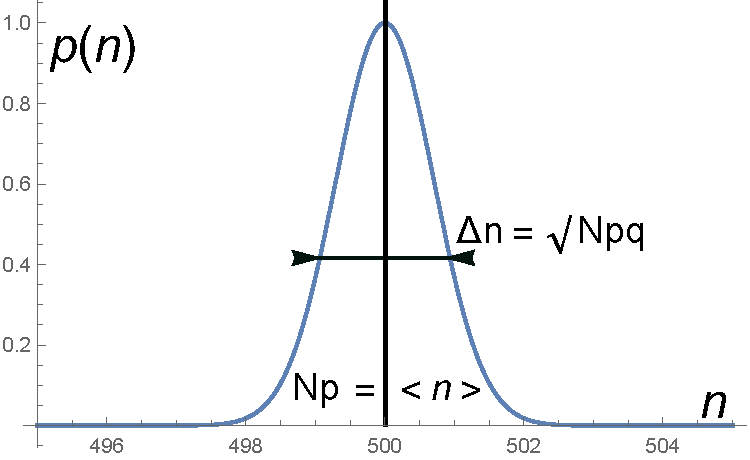
\includegraphics[width=0.5\textwidth]{graphs/gaussEex}
  \end{center}
\end{figure}

As a sanity check we compute the maximum $n^*$ of this function:
\[
\frac{\partial }{\partial n} \log(p(n)) \Bigg|_{n^*} = -\log n + \log(N-n) + \log p - \log q \Bigg|_{n^*} = 0 \Leftrightarrow \frac{n^*}{N - n^*} = \frac{p}{1 - p} \Leftrightarrow n^* = Np
\]
Now since we are dealing with small quantities we take a Taylor expansion:
\begin{align*}
\log(p(n)) &= \log(p(n^*)) + \frac{\partial}{\partial n}\log p(n) \Bigg|_{n^*}(n - n^*) + \frac{1}{2}\frac{\partial^2}{\partial n^2} \log(p(n)) \Bigg|_{n^*} (n - n^*)^2 + \cdots\\
&= \log(p(n^*)) - \frac{1}{2 N p q}(n - n^*)^2
\end{align*}
Rewriting this we get that:
\[
p(n) = A\exp\left(-\frac{1}{2Npq}\left(n - n^*\right)^2\right) \quad \text{ and normalization gives } \quad A = \frac{1}{\sqrt{2\pi N p q}}
\]
We see that $p(n)$ approaches a Gaussian as $N \to +\infty$, which also explains why the log behaved so well previously.

\section{Emergent Laws: example of a voting model.}
\begin{wrapfigure}{R}{0.15\textwidth}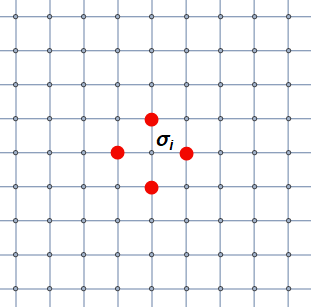
\includegraphics[width=0.15\textwidth]{graphs/SquareLattice}\end{wrapfigure}
When we take $N \to + \infty$ we are breaking symmetries of the microscopic model and behaviors arise from the collective interactions. To illustrate this we take a voting model: 'the majority vote model'.We take a finite square lattice with $N$ nodes, illustrated here. To each node we associate a parameter that can take two values: $\sigma_i = +1/-1$. We then make the system evolve by finite time steps $\Delta t$ which can correspond to a day for example. The evolution consists of each node having a probability $1-q$ of taking the majoritary opinion of its neighbors and a probability $q$ of taking the minoritary one. Now we define the following:


\[
w_i := \text{ probability that } i \text{ changes opinion} \quad S_i := \text{ neighboring opinion } = \text{sign}(\sigma_{i\uparrow} + \sigma_{i\downarrow} + \sigma_{i\leftarrow} + \sigma_{i\rightarrow})
\]
We can see case by case that we can write:
\[
w_i = \frac{1}{2}(1 - (1 - 2q)\sigma_i S_i)
\]
And note that this formula also behaves well when $S_i = 0$. The question now is how does the opinion of $i$ evolve. We know that $\sigma_i$ will stay the same with a probability $1 - w_i$ and change of $-2\sigma_i$ with probability $w_i$, so we get:
\[
\frac{\Delta \sigma_i}{\Delta t} = 0\cdot(1 - w_i) - 2\sigma_i w_i = -\sigma_i + (1 - 2q)\sigma_i^2 S_i = -\sigma_i + (1 - 2q)S_i
\]
So we get $\frac{d\sigma_i}{dt} = -\sigma_i + (1 - 2q)S_i$  with $S_i = \text{sign}\left(\sum_{k \in \mathcal{N}(i)} \sigma_k\right)$. Now let's call $m = \langle \sigma_i \rangle$ the average opinion. Furthermore, since the sign function is really bad to handle we rewrite:
\[
S_i = \frac{3}{8}(\sigma_{i\uparrow} + \sigma_{i\downarrow} + \sigma_{i\leftarrow} + \sigma_{i\rightarrow}) - \frac{1}{8}(\sigma_{i\uparrow}\sigma_{i\downarrow}\sigma_{i\leftarrow} + \sigma_{i\downarrow}\sigma_{i\leftarrow}\sigma_{i\rightarrow} + \sigma_{i\leftarrow}\sigma_{i\rightarrow}\sigma_{i\uparrow} + \sigma_{i\rightarrow}\sigma_{i\uparrow}\sigma_{i\downarrow})
\]
We leave it as an exercise to the reader to check case by case that this formula works. Now we will do what is called the 'mean field approximation' which will be justified and explained later in the notes. It simply consists of saying that every node behaves independently of everyone else, so everyone behaves more or less like the mean. More concretely we get that:
\[
\frac{d\langle \sigma_i\rangle}{dt} = -\langle \sigma_i \rangle + (1-2q)\left[ \frac{3}{8}\sum_{k \in \mathcal{N}(i)} \langle \sigma_k \rangle - \frac{1}{8}\Big( \langle \sigma_{i\uparrow}\sigma_{i\downarrow}\sigma_{i\leftarrow} + \cdots \} \Big) \right] \approx - m + (1-2q)\left[ \frac{3}{2} m - \frac{1}{2}m^3 \right]
\]
Now we call $\gamma = (1 - 2q)$ and so we write:
\[
\frac{dm}{dt} = (-1 + \frac{3}{2}\gamma)m - \frac{\gamma}{2}m^3
\]
What interests us are the stationary states, so we try and find:
\[
\frac{dm}{dt} = 0 \Leftrightarrow m(-1 + \frac{3\gamma}{2} - \frac{\gamma}{2}m^2) = 0 \Rightarrow \begin{cases}
m = 0\\
m^2 = - \frac{2\varepsilon}{\gamma}
\end{cases}
\]
Now if $\varepsilon > 0$ then $m = 0$ is the only solution, otherwise $m = 0$ and $m = \pm \sqrt{\frac{2\varepsilon}{\gamma}}$ are solutions. Furthermore $\varepsilon = 3(q - \frac{1}{6})$ so we see that the critical value is $q_c = 1/6$. It is also quite straight-forward to check that all solutions are stable with the exception of $m = 0$ when $q < q_c$.
\begin{figure}[h]
  \begin{center}
    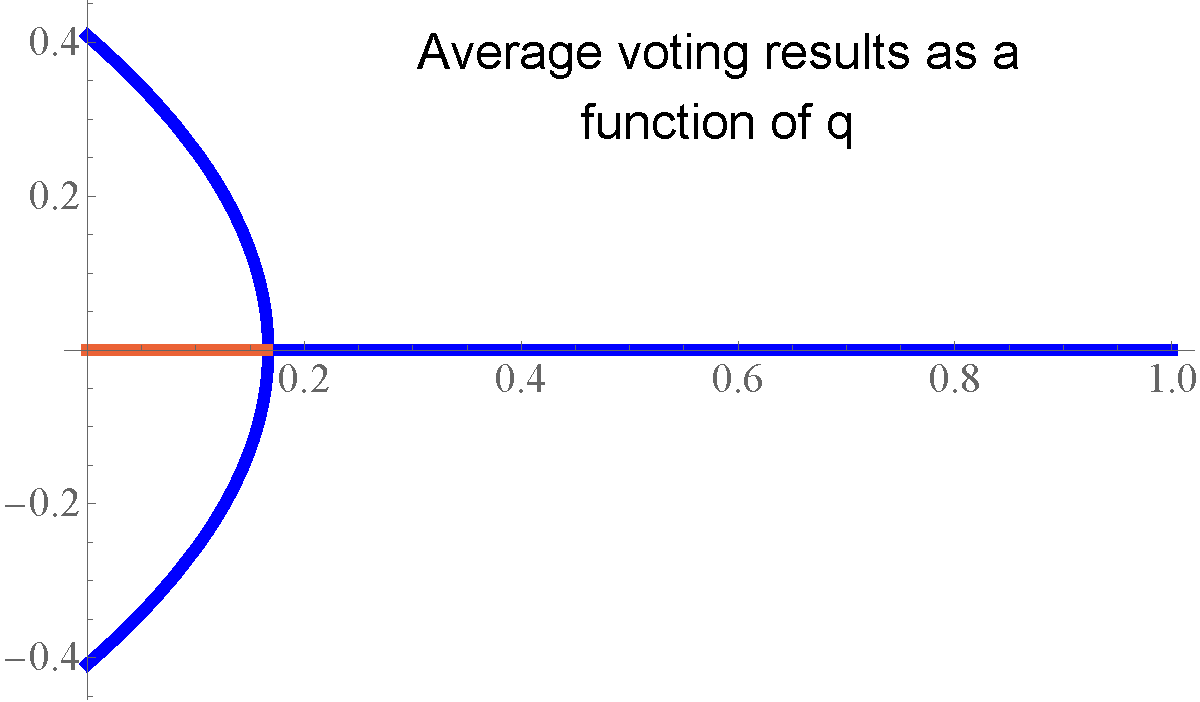
\includegraphics[width=0.4\textwidth]{graphs/voting_result}
  \end{center}
\end{figure}


\chapter{Combinatorics and emergent laws.}

In this chapter we will study perfect systems in a bit of a cheap way what will be done more rigorously later. We aim simply at giving an introduction, a taste of the type of physical problems that statistical physics can solve.

\section{Perfect Gas}
\subsection{Combinatorics of an elementary system without interactions.}
\begin{wrapfigure}{r}{0.25\textwidth}
    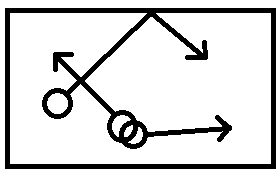
\includegraphics[width=0.25\textwidth]{graphs/GasNoCol}
\end{wrapfigure}

To start with we consider a fixed volume $V$ with a fixed number of particles $N$ that don't interact with each other, so we ignore collisions altogether. The system is also completely isolated from everything else.
Then each particle is described by two three dimensional vectors:
\[
\begin{cases}
\overrightarrow{r_i} = (x_i, y_i, z_i)(t)\\
\overrightarrow{p_i} = m(v_{x_i}, v_{y_i}, v_{z_i})(t)
\end{cases}
\]
So our problem is evolving in a $6$ dimensional phase space, call it $\Gamma$. We then subdivide this space in elementary cells of size $\Delta \Gamma$, so we write:
\[
\Gamma = \Big\{\left\{\overrightarrow{r_1}, \overrightarrow{p_1}\right\}, \left\{\overrightarrow{r_2}, \overrightarrow{p_2}\right\}, \cdots \Big\} \quad \text{ and } \quad \Delta \Gamma = (\Delta x \, \Delta y\, \Delta z\, \Delta p_x\, \Delta p_y\, \Delta p_z)
\]
The size of $\Delta \Gamma$ will be without importance in the following but we will see later that it will play a role when quantum physics intervenes. Now let $\alpha$ be a microscopic state, since the system is completely isolated we have that:
\[
\epsilon_\alpha = \frac{1}{2}mv_\alpha^2 = \frac{1}{2}\frac{p_\alpha^2}{m}
\]
Now we make the following postulate: \textbf{all the configurations of the phase space are equiprobable}. So if we have $M$ cells in total each cell has a probability of $p = \frac{1}{M}$ to be occupied by a given particle. The question we want to answer is what is the most probable configuration for our system. Similarly as in the previous chapter we get that:
\[
\mathbb{P}(n_1, n_2, \cdots, n_m) = \frac{N!}{n_1!n_2!\cdots n_m!}\left(\frac{1}{M}\right)^N
\]
And we have the following constraints:
\[
n_1 + n_2 + \cdots + n_m = N \quad \text{ and } \quad n_1\epsilon_1 + n_2\epsilon_2 + \cdots n_m \epsilon_m = E_T
\]
To maximize the probability the easiest way is to use Lagrangian multipliers (see Appendix). So we write:
\[
F := \log\mathbb{P}(n_1, \cdots, n_m) - \mu\left(\sum_{i = 1}^m n_i - N\right) - \beta\left(\sum_{i = 1}^m n_i \epsilon_i - E\right)
\]
Then using Stirling's formula we immediately get that:
\[
\frac{\partial F}{\partial n_i} = 0 = -\log n_i - \mu - \beta \epsilon_i \quad \text{ so the most probable state is } n_i = e^{-\mu - \beta\epsilon_i}
\]
Then $\mu$ and $\beta$ are fixed by the initial constraints: $N = \sum_{i = 1}^m n_i$ and $E = \sum_{i = 1}^m n_i\epsilon_i$.
\subsection{Distribution of Energy}
\subsubsection{Perfect Gas}
Let's say that we want to know how many particles in a perfect gas have a given energy: $\epsilon = \frac{1}{2}mv^2$. Then using the previous result we get that:
\[
\# \text{particles with energy } \epsilon = C \, d^3\vec{r} \,d^3 \vec{v} e^{-\beta \frac{1}{2}mv^2}
\]
Using normalization to determine $C$ we get that:
\[
\int C\, d^3 \vec{r}\, d^3 \vec{v} \, e^{-\beta \frac{1}{2}mv^2} = N \Rightarrow CV\left(\sqrt{\frac{2\pi}{\beta m}}\right)^3 = N
\]
So we get the following:
\[
\# \text{ particles with } (\vec{r}, \vec{v}) = d^3 \vec{r}\, d^3 \vec{v}\, \rho \left(\frac{\beta m}{2\pi}\right)^{3/2} \exp\big[-\beta \frac{1}{2}mv^2\big] \quad \text{ with } \rho = N/V
\]
This is what is called the Maxwell-Boltzmann distribution.
\subsubsection{Average Energy}
From the previous computation we have that the average energy will be given by:
\begin{align*}
E &= \int d^3 \vec{r} \int d^3 \vec{v}\, \left(\frac{1}{2}mv^2\right)\rho \left(\frac{\beta m}{2\pi}\right)^{3/2} \exp\left(-\beta \frac{1}{2}mv^2\right) = N\left(\frac{\beta m}{2\pi}\right)^{3/2}\int d^3 \vec{v}\, \left(\frac{1}{2}mv^2\right) \exp\left(-\frac{\beta}{2}mv^2\right)\\
(\,\cdots) &= \frac{3}{2}\frac{N}{\beta}
\end{align*}
Without any interaction we have that $E \sim T$ so $\beta \sim \frac{1}{T}$. More precisely we will see that $\beta = \frac{1}{k_B T}$ with $k_B = 1.38 \cdot 10^{-23} \, \text{J}/\text{K}$ which is the Boltzmann constant.

\subsection{Elements of cinetic theory and law of Boyle-Mariotte.}
The law of Boyle-Mariotte is:
\[
PV = Nk_BT
\]
This is what we will try to explain now using cinetic theory. Cinetic theory simply consists of taking the previous example but now taking collisions into account.
\subsubsection{Pressure}
First we want to explain microscopically what is pressure. The way we understand it here in first approximation is that when a particle bounces of a wall it will change momentum and therefore exert a force on the wall.
\begin{wrapfigure}{r}{0.25\textwidth}
  \begin{center}
    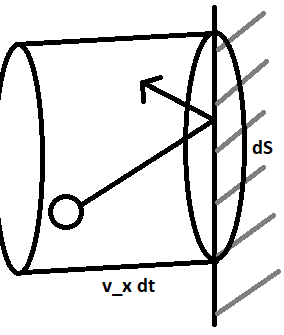
\includegraphics[width=0.22\textwidth]{graphs/PressureDiag}
  \end{center}
\end{wrapfigure}
More precisely we have:
\[
(\Delta \vec{p})_x = -2 m v_x \quad \text{ so } \quad \vec{F}_\text{wall} = \langle\frac{\Delta p}{\Delta t}\rangle
\]
Now on a given time step $\Delta t$ we need to determine how many particles are colliding with the wall. Assuming that all particles maintain the same velocity in this time step $\Delta t$ we can see geometrically that all the particles found in the cylinder of base $\Delta S$ and height $v_x\Delta t$ will collide (with $v_x > 0$).
Then we get that (call $f$ the Maxwell-Boltzmann distribution):
\[
dF_x = -\int_{v_x > 0} d^3\vec{v}\, \frac{\Delta p_x}{\Delta t}(v_x \Delta t \, dS) C f(\vec{v}) \quad \text{ so } \quad P = \frac{dF_x}{dS} = \rho \int_{v_x > 0} d^3 \vec{v}\, 2mv_x^2 f(\vec{v})
\]
Now notice that this is just another way of writing an average value, so we have that:
\[
P = \rho \langle 2m v_x^2 \rangle_{v_x > 0}
\]
We know want to compute what is $\langle v_x^2 \rangle_{v_x > 0}$. To do so we make the equipartition assumption. This consists of saying that energy is equally subdivided in each degree of freedom of the system. So we get the following:
\[
\begin{cases}
\frac{E}{N} = \frac{1}{2}m \langle v^2 \rangle = \frac{3}{2}\frac{1}{\beta}\\
\langle v_x^2 \rangle = \frac{1}{3} \langle v^2 \rangle\\
\langle v_x^2 \rangle_{v_x > 0} = \langle v_x^2 \rangle 
\end{cases}
\quad  \text{ so } \quad \langle v_x^2\rangle_{v_x > 0} = \frac{1}{2\beta m}
\]
Plugging this back in the equation we have for the pressure we get that:
\[
P = 2m\langle v_x^2 \rangle_{v_x > 0} \rho = \frac{\rho}{\beta} \Leftrightarrow PV = \frac{N}{\beta} \Leftrightarrow PV = Nk_B T
\]
\subsubsection{Ambient air example}
Applying what we just saw to ambient air where the pressure is of approximately $P = 10^5 \text{ Pa}$ we get that:
\[
v \sim \sqrt{\frac{k_B T}{m}} \sim 10^2 \text{ m}/\text{s} \quad \text{ and } \quad \frac{\Delta P}{P} = \frac{\Delta N}{N} \sim \frac{1}{\sqrt{N}} \sim 10^{-13}
\]
So we see that the force exerted on a $1\text{m}^2$ window is of $10^5$ Newtons. Although this might seem huge one has to remember that the same force is exerted on all sides, which explains why the window isn't exploding. Furthermore we see that the fluctuations will exert only up to a force of the order of $10^{-8}$ N, which clearly is not enough to break windows. In a way we are very lucky that fluctuations are so small otherwise life would be a bit more complicated.

\subsection{Barometric Law}
We now consider the same problem but we now add gravity (or any other time-independent potential). The modification is quite easy to make, it suffices to change the energy of a cell as follows:
\[
\epsilon_i = \frac{1}{2}mv_i^2 + V(\vec{r}) = \frac{1}{2}mv_i^2 + mgz_i
\]
Then the Maxwell-Boltzmann distribution is re-written as follows:
\[
\# \text{ particles with } (\vec{r}, \vec{v}) \propto \exp\Big[ -\beta\left( \frac{1}{2}mv^2 + mgz \right) \Big]
\]
And so we get that:
\[
\rho(z) = \rho_0 \exp(-\beta m g z)
\]
If we compute this with the usual balance of forces method from mechanics we get the same result:
\[
0 = -P(z+dz)dS + P(z)\,\text{d}S - \rho m g \, \text{d}S\, \text{d}Z = -\frac{\partial P}{\partial z} \,\text{d}S\, \text{d}z - \rho mg\, \text{d}S \, \text{d}z
\]
So we get that:
\[
\begin{cases}
\frac{\partial P}{\partial z} = - \rho m g\\
P = \rho k_B T
\end{cases}
\Rightarrow \frac{\partial \rho}{\partial z} = - \frac{mg}{k_B T}\rho \Rightarrow \rho = \rho_0 \exp\left[-\frac{mgz}{k_B T}\right]
\]


\section{Ideal Polymers}
[...]
\subsection{Statistics}
\subsection{Probability and Mechanics}


\subsection{Introduction to the notions of statistical ensembles and fundamental postulate.}
\subsubsection{Generalizations}
The ensembles of statistical physics that we are going to study in the following are the micro-canonical ensemble, where $N, V, E$ are fixed so isolated systems. The next one is the canonical ensemble where $N, V, T$ are fixed. Finally we will study the grand-canonical ensemble where $\mu, V, T$ are fixed.

[...]

We take a system of $N$ particles then our system is described by $2N$ vectors: $\overrightarrow{r_i}(t)$, $\overrightarrow{v_i}(t)$. Or equivalently with $2N$ canonical variables: $\overrightarrow{q_i}(t)$, $\overrightarrow{p_i}(t)$. We then introduce the Hamiltonian $\mathcal{H}(\{\overrightarrow{q_i}, \overrightarrow{p_i}\}, t)$, then the equations of motion of our system are:
\[
\begin{cases}
\dot{\overrightarrow{q_i}} = \frac{\partial \mathcal{H}}{\partial \overrightarrow{p_i}}\\
\dot{\overrightarrow{p_i}} = - \frac{\partial \mathcal{H}}{\partial \overrightarrow{q_i}}
\end{cases}
\]
We then introduce the density $\rho(\{\overrightarrow{q_i}, \overrightarrow{p_i}\}, t)$ and if we have:
\[
\mathcal{H} = \frac{1}{2}\frac{\overrightarrow{p}^2}{m} + V(\overrightarrow{q}) \quad \text{ then we get that } \quad \dot{\overrightarrow{q_i}} = \frac{\partial \mathcal{H}}{\partial \overrightarrow{p}} = \frac{\overrightarrow{p}}{m}
\]
We then introduce the phase space $\Gamma = \{\overrightarrow{q_i}, \overrightarrow{p_i}\}$ and subdivide it in base elements $\dd\Gamma = \prod_{i = 1}^N \text{d}\overrightarrow{q_i}\text{d}\overrightarrow{p_i}$.
\subsubsection{Strum-Lioumville equation.}
Note that we can write:
\[
\rho(\Gamma, t) = \prod_{i = 1}^N \delta(\overrightarrow{q_i} - \overrightarrow{q_i}(t))\delta(\overrightarrow{p_i} - \overrightarrow{p_i}(t))
\]
Note also that:
\[
\frac{\partial}{\partial t}\delta(x - x(t)) = -\frac{\partial x}{\partial t}\delta'(x - x(t)) = - \dot{x}\grad_x \delta(x - x(t))
\]
Applying this to the above definition of the density we get that:
\begin{align*}
\frac{\partial \rho}{\partial t} = \sum_i \Big(-\frac{\partial \overrightarrow{q_i}}{\partial t} \Big)\Big( \grad_{q_i} &\delta(\overrightarrow{q_i} - \overrightarrow{q_i}(t)) \delta(\overrightarrow{p_i} - \overrightarrow{p_i}(t)) \Big)\prod_{j = 1}^N \delta(\overrightarrow{q_j} - \overrightarrow{q_j}(t))\delta(\overrightarrow{p_j} - \overrightarrow{p_j}(t)) \\
&+ \Big(-\frac{\partial\overrightarrow{p_i}}{\overrightarrow{\partial t}}\Big)\Big( \grad_{q_i} \delta(\overrightarrow{q_i} - \overrightarrow{q_i}(t)) \delta(\overrightarrow{p_i} - \overrightarrow{p_i}(t)) \Big)\prod_{j = 1}^N \delta(\overrightarrow{q_j} - \overrightarrow{q_j}(t))\delta(\overrightarrow{p_j} - \overrightarrow{p_j}(t))
\end{align*}
We then can rewrite this as:
\[
\frac{\partial \rho}{\partial t} = -\left( \sum_i \dot{\overrightarrow{q_i}} \grad_{q_i} \rho + \dot{\overrightarrow{p_i}}\grad_{p_i} \rho\right) = - \sum_i \left(\frac{\partial \rho}{\partial \overrightarrow{q_i}}\frac{\partial \mathcal{H}}{\partial \overrightarrow{p_i}} - \frac{\partial \rho}{\partial \overrightarrow{p_i}}\frac{\partial\mathcal{H}}{\partial \overrightarrow{q_i}}\right)
\]
We then introduce what is called the Poisson bracket:
\[
\{A, B\} = \sum_i \left( \frac{\partial A}{\partial \overrightarrow{q_i}} \frac{\partial B}{\partial \overrightarrow{p_i}} - \frac{\partial A}{\partial \overrightarrow{p_i}} \frac{\partial B}{\overrightarrow{q_i}} \right)
\]
We can then write the Strum-Liouville equation:
\[
\frac{\partial \rho}{\partial t} = \{\mathcal{H}, \rho\}
\]
Remark that we can re-write:
\[
\frac{\partial \rho}{\partial t} = - \sum_i \grad_{q_i}(\dot{\overrightarrow{q_i}} \rho) + \grad_{p_i}(\dot{\overrightarrow{p_i}}\rho)
\]
Since
\[
(\grad_{q_i}\dot{\overrightarrow{q_i}} + \grad_{p_i}\dot{\overrightarrow{p_i}})\rho = \left(\frac{\partial^2 \mathcal{H}}{\partial \overrightarrow{q_i}\partial\overrightarrow{p_i}}  - \frac{\partial^2 \mathcal{H}}{\partial \overrightarrow{q_i}\partial\overrightarrow{p_i}}\right)\rho = 0
\]
This then gives:
\[
\frac{\partial \rho}{\partial t} = - \grad (\overrightarrow{v} \rho)
\]
Which shows that probabilities are conserved. An important result of this is that any function that depends only of $\mathcal{H}$ is a stationary solution of the Liouville equation, or in mathematics terms:
\[
\rho(\mathcal{H}) \quad \text{ verifies } \quad \frac{\partial \rho}{\partial t} = \{\mathcal{H}, \rho\} = 0
\]
\subsubsection{Ensembles and postulate.}
What we want to do is to move from a microscopically dynamic system to a probabilistic one. The idea behind how to do so is to take the phase space, then instead of looking at one set of initial condition we look at $M$ initial conditions. Then in each element of the phase space we give a density of probability corresponding to the average presence of the paths given from the initial conditions, i.e:
\[
\rho(\Gamma) = \frac{1}{M}\sum_\alpha \rho_\alpha (\Gamma)
\]
We then define averages like:
\[
\langle A \rangle = \int \text{d}\Gamma \rho(\Gamma)A(\Gamma)
\]
\subsubsection{Ensembles.}
Statistical physics is divided in multiple ensembles. We are going to see:
\begin{itemize}
\item The micro-canonical ensemble: the energy of the system is fixed and the system is isolated, so $N$ and $V$ don't vary either.
\item The canonical ensemble: Instead of fixing the energy we know fix the temperature. So $N,V,T$ are fixed.
\item The grand-canonical ensemble: we fix the chemical potential instead of the number of particles. So $\mu, V, T$ are fixed.
\end{itemize}
\subsubsection{Fundamental Postulate.}
\begin{center}
In an isolated system at equilibrium all the microscopic states are equally probable.
\end{center}
Remark that this means that at equilibrium $\rho_{\text{eq}}(\Gamma)$ becomes independent of $\Gamma$ and we have instead that:
\[
\rho_{\text{eq}} = \frac{1}{\# \text{nb. of microscopic states}}
\]
Which, as we will see, depends of $E$. Notice as well that this agrees with the microscopic dynamics since it satisfies the Liouville equation. If $\rho$ depends only of $E$ it can be written as a function of $\mathcal{H}$ and so is a stationary solution of the Liouville equation.

\chapter{Microcanonical ensemble.}
Once more, in the microcanoncal ensemble we look only at problems where the system is isolated, the energy, the volume and the number of particles are fixed.
\section{Microcanonical partition function.}
We made the following postulate:
\[
\rho_{\text{eq}} (\Gamma) = \frac{1}{\Omega} \quad \text{ where } \quad \Omega = \# \text{ microstates of energy } E
\]
Another way to write this is:
\[
\Omega = \sum_{\text{microstates } s| N(s) = N, V(s) = V, E(s) = E} 1
\]
Now to simplify calculus we introduce an uncertainty on the energy $\Delta E$. So instead of requiring a strict equality we know require that $E \leq \mathcal{H}(\Gamma) \leq E + \Delta E$. Although not obvious at first we will see that in the end $\Delta E$ has no impact on the physics and is simply a calculus trick. We also define the average of a quantity as:
\[
\langle A \rangle = \int \dd\Gamma A(\Gamma)\rho(\Gamma) = \frac{\int_{E \leq \mathcal{H}(\Gamma) \leq E + \Delta E} \dd \Gamma A(\Gamma)}{\int_{E \leq \mathcal{H}(\Gamma) \leq E + \Delta E} \dd \Gamma 1}
\]
We now introduce the partition function. Take our phase space, then we subdivide it in such a way that:
\[
\Delta \overrightarrow{q_{i}} \Delta \overrightarrow{p_{i}} = h^3 \quad \text{ where } h \text{ is Planck's constant.}
\]
Now instead of summing on all of our microstates as we did before we are going to use this subdivision and re-write:
\begin{equation}
\Omega = \frac{1}{N!} \int_{E \leq \mathcal{H}(E) \leq E + \Delta E} \frac{\dd \Gamma}{h^{3N}}1
\end{equation}
This is the partition function, note that we artificially add the $N!$ term because our integral does not take into consideration the undiscernability of the particles. Note though that the adding of this $N!$ is not trivial at all\footnote{It is so subtle that it is still being discussed: D. Frenkel, Molecular Physics, 112 2325 (2014)}.

\section{Entropy and Temperature.}
We define the entropy, as done by Boltzmann in 1872, by:
\begin{equation}
S = k_B \log\Omega \quad \text{ with } k_B \text{ being the Boltzmann constant.}
\end{equation}
Then the temperature is defined by:
\[
\frac{1}{T} = \pdv{S}{E}\Bigg|_{V,N}
\]
We will see this more in detail later, but we just mention that the entropy is an extensive variable and $T$ is an intensive variable so when we consider two systems 1, 2 we have:
\[
S_{1 \cup 2} = S_1 + S_2 \quad \text{ while } \quad T_{1 \cup 2} = T_1 = T_2
\]

\section{Entropy of the perfect gas.}
A perfect gas is a gas with no interactions, which translates to:
\[
\mathcal{H}(\Gamma) = \sum_{i = 1}^N \frac{\overrightarrow{p_i}^2}{2m}
\]
Now what we have to compute is:
\[
\Omega = \frac{1}{N!}\frac{1}{h^{3N}}\int_{E \leq \sum_{i = 1}^N\frac{\overrightarrow{p_i}^2}{2m} \leq E + \Delta E} \dd\Gamma
\]
We then decompose $\dd\Gamma$ in its two fundamental building blocks and use the fact that the positions are independent of the energy. We then get:
\[
\Omega = \frac{1}{N!}\frac{1}{h^{3N}}\int_{V\times V\times\cdots} \dd\overrightarrow{r_1}\cdots\dd\overrightarrow{r_N}\int_{2mE \leq \sum_i \overrightarrow{p_i}^2 \leq E + \Delta E} \dd\overrightarrow{p_1} \cdots \dd\overrightarrow{p_N} = \frac{V^N}{N! h^{3N}} \Delta \mathcal{V}(E)
\]
Now we need to compute that last term:
\[
\Delta \mathcal{V}(E) = \int_{2mE \leq \sum_i \overrightarrow{p_i}^2 \leq E + \Delta E} \dd \overrightarrow{p_1}\cdots\dd\overrightarrow{p_N}
\]
To do so we use our $\Delta E$ term in the following way, we say that:
\[
\mathcal{V}(E) = \int_{0 \leq \sum_i \overrightarrow{p_i}^2 \leq 2mE} \quad \text{ and } \quad \Delta \mathcal{V}(E) = \mathcal{V}(E + \Delta E) - \mathcal{V}(E)
\]
Note that this corresponds simply to the volume of a hyper-sphere of dimension $3N$, for which we know the explicit formula:
\[
\mathcal{V}(E) = \frac{\pi^{\frac{3N}{2}}}{(\frac{3N}{2})!}R^{3N} \quad \text{ with } \quad R = \sqrt{2mE}
\]
Then we write:
\[
\Delta \mathcal{V} = \mathcal{V}(E + \Delta E) - \mathcal{V}(E) \approx \Delta E \mathcal{V}'(E) \quad \text{ with } \quad \mathcal{V}'(E) = \frac{\pi^{\frac{3N}{2}}}{(\frac{3N}{2})!} \frac{3N}{2} \frac{(2mE)^{\frac{3N}{2}}}{E}
\]
We can then deduce that:
\[
\Omega = \frac{V^N}{N!h^{3N}} \frac{\pi^{\frac{3N}{2}}}{(\frac{3N}{2})!}(2mE)^{\frac{3N}{2}}\frac{\frac{3N}{2}N\Delta E}{E}
\]
We can now compute the entropy of our system:
\[
S = k_B\log\Omega
\]
And if we write $\Omega = \omega^N \frac{3N\Delta E}{E}$ we then get:
\[
\log\Omega = N\log \omega + \log(\frac{3N\Delta E}{E}) \approx N\log\omega
\]
Now more precisely:
\begin{align*}
S \approx k_B \log \left[ \frac{V^N}{N! h^{3N}} \frac{\pi^{\frac{3N}{2}}}{(\frac{3N}{2})!} (2mE)^{\frac{3N}{2}} \right] &= k_B N \left( \log V \left( \frac{2\pi m E}{h^2} \right)^{\frac{3}{2}} - \log N + 1 - \frac{3}{2}\log N + \frac{3}{2} \right)\\
&= k_B N\left( \log\left( \frac{V}{N}\left(\frac{\frac{4\pi}{3}mE/N}{h^2}\right)^{3/2} \right) \right) + \frac{5}{2}
\end{align*}
This is what is called the Sackur-Tetrode formula. We now introduce a few variables:
\begin{itemize}
\item $\rho = \frac{N}{V}$, the numeric density not to be confused with our previous $\rho$ of $\Gamma$.
\item $\lambda = \sqrt{\frac{h^2}{\frac{4\pi}{3}m \frac{E}{N}}}$ which is called the De Broglie wavelength.
\end{itemize}
As an aside, know that the De Broglie wavelength indeed has the unit of a length and actually corresponds to the length under which quantum effects dominate and become non-negligible. For a perfect gas at 300K this gives $\lambda \sim 10^{-11} \text{m}$, and the distance in between particles $\frac{1}{\rho^{1/3}} \sim \text{nm} \gg \lambda$. Now re-writing the formula we have:
\begin{equation}
S = k_B N \left(\log\frac{1}{\rho\lambda^3} + \frac{5}{2}\right)
\end{equation}
Note that if we had not included the $N!$ term earlier we would not have gotten $\rho$ here and therefore the entropy would not behave as an extensive variable.
\subsubsection{Temperature}
Now that we have the entropy we can try and compute the temperature. We have the formula:
\[
\frac{1}{T} = \pdv{S}{E}\Bigg|_{V,N} \quad \text{ and } \quad S = k_B N\left(\log(\alpha E^{3/2}) + \frac{5}{2}\right)
\]
This then gives:
\[
\frac{1}{T} = \pdv{S}{E}\Bigg|_{N,V} = k_B N \frac{3}{2E} \Rightarrow E = \frac{3}{2}Nk_B T
\]

\section{General Properties of Entropy.}
\subsection{Evolution towards equilibrium: increase of entropy.}
\begin{wrapfigure}{r}{0.25\textwidth}
    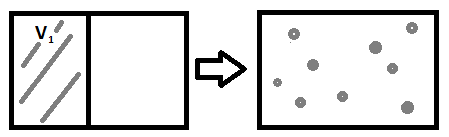
\includegraphics[width=0.25\textwidth]{graphs/ChangeEx}
\end{wrapfigure}
We are as always considering an isolated system where at $t = 0$ we add a constraint '$x$'. When we remove the constraint the number of possible microstates increases so:
\[
\Omega_f \geq \Omega_i \quad \text{ so } \quad S_f \geq S_i \quad \text{ and } \quad \Delta S \geq 0
\]
Then a general property that we are going to look at now is that the equilibrium is found by maximizing the entropy.

\subsection{Thermodynamic equilibrium.}
\begin{wrapfigure}{r}{0.25\textwidth}
    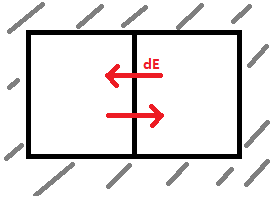
\includegraphics[width=0.25\textwidth]{graphs/thermo_eq}
\end{wrapfigure}
We consider the following system: we take a fixed isolated volume and separate it in two systems $V_1, N_1, E_1$ and $V_2, N_2, E_2$ separated by an impermeable barrier. However energy can be exchanged in between the two systems. So we have $V_1, V_2$ and $N_1, N_2$ constant, and $E = E_1 + E_2$ constant.

Then the number of microstates is given as follows:
\[
\Omega = \Omega_1 \times \Omega_2
\]
So we have that:
\[
S_{1 \cup 2} = k_B \log \Omega = k_B \log\Omega_1 + k_B \log \Omega_2 \Rightarrow S_{1 \cup 2} = S_1 + S_2
\]
We now look for the equilibrium. So we are trying to maximize the following function:
\[
S_{1 \cup 2} (E_1, E_2 = E - E_1, V_1, V_2, N_1, N_2) = S_1(E_1) + S_2(E - E_1)
\]
We see immediately that we need to maximize for $E_1$ so:
\[
\text{equilibrium} = \max_{E_1} S(E_1)
\]
So we solve:
\[
0 = \pdv{}{E_1} S_{1 \cup 2} = \pdv{S_1}{E_1}\Bigg|_{\text{eq}} - \pdv{S_2}{E_2}\Bigg|_{\text{eq}} = \frac{1}{T_1} - \frac{1}{T_2} \Rightarrow T_1 = T_2
\]
\subsubsection{Alternative method.}
We now show another way to solve this problem because we want to stress a certain solving technique. First we write:
\[
\Omega(E) = \sum_{E_1} \Omega_1(E_1)\Omega_2(E - E_1) = \int \frac{\dd E_1}{\Delta E} \Omega_1(E_1)\Omega_2(E - E_1) = \int \frac{\dd E_1}{\Delta E_1} e^{\frac{S_1(E_1)}{k_B} + \frac{S_2(E - E_1)}{k_B}} 
\]
But notice that the integrand is simply gigantic. The terms in the exponential are of the order of $N \sim 10^{23}$ and since the exponential is a fast varying function, this integrand is extremely spiked at its maximum value. We therefore consider that the integral is dominated by the values close to the maximum of the integral. This is what we call the method of steepest descent. So now, what is the maximum of the integral? To answer this we have to maximize:
\[
\max_{E_1} S_1(E_1) + S_2(E - E_1) \Rightarrow \frac{1}{T_1} = \frac{1}{T_2}
\]
Denote $E_1^*$ the value for which the maximum is reached. Now we write:
\[
S_1 + S_2 = S_1(E_1^*) + S_2(E - E_1^*) + \pdv{}{E_1}\left(S_1 + S_2\right)\Bigg|_{E_1^*} (E_1 - E_1^*) + \frac{1}{2} \pdv[2]{}{E_1} \left(S_1 + S_2\right)\Bigg|_{E_1^*}(E_1 - E_1^*)^2
\]
Then plugging this back in we get:
\[
\Omega(E) = e^{\frac{S_1(E_1^*) + S_2(E - E_1^*)}{k_B}} \int \frac{\dd E_1}{\Delta E} e^{\frac{1}{2k_B} \pdv[2]{(S_1+S_2)}{E_1}\Big|_{E_1^*} (E_1 - E_1^*)^2}
\]
This is a Gaussian integral that we know how to compute and we get that:
\[
\Omega(E) = e^{\frac{S}{k_B}} \sqrt{\frac{2\pi k_B}{\Big| \pdv[2]{S}{E_1}\big|_{E_1^*}\Big |} }
\]
Note that we need to take the absolute value because since we are at a maximum the function will be concave and the second derivative negative. Now we write:
\[
S_\text{eq} = k_B \log \Omega = \underbrace{S_1(E_1^*) + S_2(E - E_1^*)}_{\sim N} + \overbrace{\log \sqrt{\frac{2\pi k_B}{\Big| \pdv[2]{S}{E_1}\big|_{E_1^*}\Big |} }}^{\sim \log N}
\]
So in the thermodynamic limit we get:
\[
S_\text{eq} = S_1(E_1^*) + S_2(E - E_1^*) \quad  \text{ with } E_1^* \text{ such that } \quad \frac{1}{T_1} = \frac{1}{T_2}
\]

\subsection{Pressure and chemical potential.}
If we write what we found previously under differential form we see that:
\[
\dd S = \frac{1}{T} \dd E \quad \text{ when all the other parameters are fixed.}
\]
We introduce a state parameter $X$ that we can make vary. Then we define the thermal forces $F$ conjugate to $X$ by the following relation:
\[
\dd S = - \frac{F}{T} \dd X \quad \text{ so equivalently } \quad F = - T \pdv{S}{X}\Bigg|_{\text{other parameters fixed}}
\]
We will see that this formula is very general and identifies well with the standard expression for pressure and other forces. Now we write:
\[
\dd S = \frac{1}{T} \dd E - \sum_\alpha \frac{F_\alpha}{T} \dd X_\alpha \quad \text{ or equivalently } \quad \dd E = T \dd S + \sum_\alpha F_\alpha \dd X_\alpha
\]
\subsubsection{Pressure.}
If we say that we can make the volume vary, we have $X = V$ and we expect to get pressure as a conjugate force: $\delta W = - P \dd V$. Indeed we get the expected formula:
\[
P = -T \pdv{S}{V}\Bigg|_{E, N} \Rightarrow \dd E = T \dd S - P \dd V
\]
\subsubsection{Chemical potential.}
The chemical potential is a force that comes from the fact that the number of particles can vary. So we have $X = N$ then:
\[
F = \mu = -T \pdv{S}{N}\Bigg|_{E, V}
\]
So we can write:
\[
\dd E = T \dd S - P \dd V + \mu \dd N
\]
\subsubsection{Equilibrium.}
When we studied the previous system we only made the energy vary, but we could make the number of particles vary as well as the volume. Then we have that:
\[
S = S_1 + S_2 = S_1(E_1, V_1, N_1) + S_2(E - E_1, V - V_1, N- N_1)
\]
Then to maximize the entropy we have to cancel all the partial derivatives:
\begin{align*}
\pdv{S}{E_1}\Bigg|_{\text{eq}} = 0 \Rightarrow \frac{1}{T_1} - \frac{1}{T_2} = 0\\
\pdv{S}{V_1}\Bigg|_{\text{eq}} = 0 \Rightarrow \frac{P_1}{T_1} - \frac{P_2}{T_2} = 0\\
\pdv{S}{N_1}\Bigg|_\text{eq} = 0 \Rightarrow -\frac{\mu_1}{T_1} + \frac{\mu_2}{T_2} = 0
\end{align*}
So at equilibrium we require that:
\[
T_1 = T_2 \quad \text{ and } \quad P_1 = P_2 \quad \text{ and } \quad \mu_1 = \mu_2
\]

\subsection{Back to the perfect gas.}
Now back to the perfect gas, we have that:
\[
S = k_B N \left( \log \left[\frac{V}{N} \left(\frac{4\pi m E}{3 N h^2}\right)^{3/2} \right] + \frac{5}{2} \right)
\]
And applying the definitions we get that:
\begin{align*}
E &= \frac{3}{2} N k_B T\\
P &= \frac{N}{V} k_B T\\
\mu &= k_B T \log(N \lambda^3) \quad \text{ where } \quad  \lambda = \sqrt{\frac{h^2}{2\pi m k_B T}}
\end{align*}
\subsection{Back to perfect polymers}
\section{The Gibbs Paradox and N!}

\chapter{Canonical Ensemble.}
The canonical ensemble in one word is that we do not want to fix the energy anymore but we fix the temperature. The reason why we want to do this is that it is much more practical since most of the time realistic systems will have a fixed temperature but not a fixed energy. There is also a technical reason which is that the math works out much more easily in this ensemble.

\section{Principles and canonical probabilities.}
\begin{wrapfigure}{r}{0.25\textwidth}
    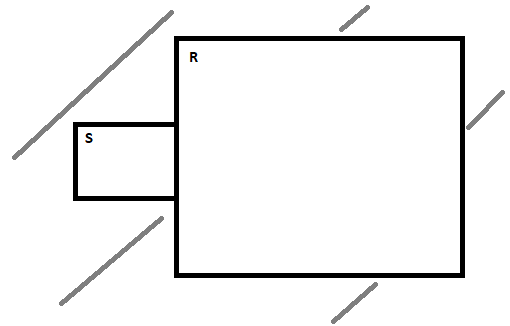
\includegraphics[width=0.25\textwidth]{graphs/sandr}
\end{wrapfigure}
The postulate of the canonical ensemble is still the same:
\begin{center}
In an isolated system all the microstates are equiprobable.
\end{center}
To model a system of the canonical ensemble what we do is we consider a system $S$ connected to a huge reservoir $R$ which are isolated from the rest. Since the reservoir is huge we consider it always at equilibrium since fluctuation in $S$ will negligibly influence $R$. We set $T_0$ to be the temperature of the reservoir then:
\[
E_{S + R} = E_S + E_R
\]
Now we want to find what is the probability of a microstate $s$ of the system $S$ at an energy $E_s$. Then:
\[
p_s = \frac{\Omega_{R} (E_R = E_\text{tot} - E_s) }{\Omega_\text{tot}}
\]
Then we have that:
\[
\Omega_R(E_\text{tot} - E_s) = \exp \left[ \frac{S_R}{k_B}(E_\text{tot} - E_s) \right]
\]
Now since $S \ll R$ then $E_s \ll E_\text{tot} \sim E_R$ so we develop and write:
\[
S_R(E_\text{tot} - E_s) \approx S_R(E_\text{tot}) - \underbrace{\pdv{S_R}{E}\Bigg|_{\text{eq}}}_{\frac{1}{T_0}} E_S + \cdots 
\]
So we get that:
\[
p_s = \frac{1}{Z}\exp(-\frac{E_s}{k_B T_0}) \quad \text{ this is called the equation of Boltzmann Gibbs}
\]
Then from normalization we need to have:
\[
Z = \sum_s \exp(-\frac{E_s}{k_B T_0})
\]
Which is what we call the partition function.

\section{Canonical partition function and Free Energy.}
The free energy is defined as being $F = E - T S$ with $T = T_0$. What we will now show is that $F = -k_B T \log Z$. First we want to compute what is the probability that the system $S$ has an energy $\dd E$ close to $E$ which we denote $p(E) \dd E$. We are doing something similar to what was done previously for the micro-canonical ensemble. Then:
\[
p(E) \dd E = \frac{1}{Z}e^{-\frac{E}{k_B T_0}} \underbrace{\omega(E)}_{\text{\# microstates of energy} E} \dd E
\]
Then from definition we have that:
\[
\omega(E) = e^\frac{S(E)}{k_B}
\]
As an aside note that $\omega$ is what is called the degeneracy in quantum mechanics, i.e. the number of states associated to a given energy. Then plugging this back in we get that:
\[
p(E) \dd E = \frac{1}{Z} e^{-\frac{E - T_0 S(E)}{k_B T_0}} \dd E \quad \text{ and } \quad \int p(E)\dd E = 1 
\]
So we get:
\[
Z = \int \dd E e^{-\frac{E - T_0 S(E)}{k_B T_0}}
\]
Now as previously we are going to use the steepest descent method. We say that the integral is dominated by the maximum of the integrand so to compute the maximum of $Z$ it suffices to compute:
\[
\min_E (E - T_0 S(E)) \quad \text{ we introduce } \quad f(E) = E - T_0 S(E)
\]
So to compute the maximum we derivate with respect to $E$ and we get that:
\[
0 = \pdv{f}{E} = 1 - T_0 \pdv{S}{E}\Bigg|_{E^*} = 1 - \frac{T_0}{T_s} \Rightarrow T_s = T_0
\]
Now we write:
\[
f(E) = f(E^*) + \cancelto{0}{f'(E^*)} (E - E^*) + \frac{1}{2} f''(E^*) (E - E^*)^2
\]
Plugging this back in we get:
\[
Z = \int \dd E e^{-\frac{E^* - T_0 S(E^*)}{k_B T_0}} e^{-\frac{1}{2} \frac{f''(E^*)}{k_B T_0} (E - E^*)^2} = e^{-\frac{E^* - T_0 S(E^*)}{k_B T_0}} \sqrt{\frac{2\pi k_B T_0}{f''(E^*)}}
\]
So approximating in the thermodynamic limit we have:
\[
-\log Z = \frac{(E - TS)\Big|_{\text{eq}}}{k_B T_0} + \mathcal{O}(\log N) \approx \frac{(E - TS)\Big|_{\text{eq}}}{k_B T_0}
\]
Then we set:
\[
F = E - TS \Big|_\text{eq} = - k_B T \log Z \quad \text{ where } T = T_0
\]
Note that for discrete systems we write:
\[
Z = \sum_s e^{-\frac{E_s}{k_B T}}
\]
But for continuous ones we write:
\[
Z = \frac{1}{N!} \frac{1}{h^{3N}} \int \dd \Gamma e^{-\frac{\mathcal{H}(\Gamma)}{k_B T}}
\]

\section{Fluctuations and thermodynamics.}
For now we have always looked at the peak of functions and neglecting the small variations around them. Now we will ask ourselves what these fluctuations are. From the previous computation we have that:
\[
p(E) \propto e^{- \frac{1}{2k_B T_0} f''(E^*)(E - E^*)^2}
\]
So we get that:
\[
\langle (\Delta E)^2 \rangle = \int \dd E (E - E^*)^2 p(E) = \frac{\int \dd E (E - E^*)^2 e^{- \frac{1}{2k_B T_0} f''(E^*)(E - E^*)^2} }{\int \dd E e^{- \frac{1}{2k_B T_0} f''(E^*)(E - E^*)^2}}
\]
Now we make a more general mathematical aside. We often have to compute quantities that have this form, and note that:
\[
\langle x^2 \rangle = \frac{\int \dd x e^{-\alpha x^2} x^2}{\int \dd x e^{-\alpha x^2}} = \frac{-\pdv{}{\alpha} \int \dd x e^{-\alpha x^2}}{\int \dd x e^{-\alpha x^2}} = -\pdv{}{\alpha} \log \underbrace{\int \dd x e^{-\alpha x^2}}_{\sqrt{\frac{\pi}{\alpha}}} = \frac{1}{2 \alpha}
\]
Now if we apply this to our case we have $x = E - E^*$ and $\alpha = \frac{1}{2k_B T_0}f''(E^*)$. So we get that:
\[
\langle (\Delta E)^2 \rangle = \langle (E - E^*)^2 \rangle = \frac{k_B T_0}{f''(E^*)}
\]
It remains only to compute $f''$ and we have:
\[
f'' = \pdv[2]{}{E} \left(E - T_0 S(E)\right) = 0 - T_0 \pdv[2]{S}{E}\Bigg|_\text{eq} = - T_0 \pdv{}{E} \left(\frac{1}{T}\right) = \frac{T_0}{T_\text{eq}^2} \pdv{T}{E}\Bigg|_{\text{eq}} \quad \text{ where } T_\text{eq} = T_0
\]
We also introduce a new variable:
\[
C_v = \pdv{E}{T}\Bigg|_{\text{eq}}
\]
Then we get that:
\[
\langle \Delta E^2 \rangle = k_B T_0^2 C_V
\]
Now to check our previous approximations we compute:
\[
\frac{\Delta E}{E} \sim \frac{\sqrt{\langle \Delta E^2 \rangle}}{E} \sim \frac{\sqrt{kT^2 C_V}}{E} \sim \frac{1}{\sqrt{N}} \rightarrow 0 
\]
\subsubsection{Another way to compute this}
Another way to compute the above is to use the probability of a microstate. We have that:
\[
p_s = \frac{1}{Z} e^{-\frac{E_s}{k_B T}} \quad \text{ with } \quad Z = \sum_S e^{- \frac{E_s}{k_B T}}
\]
So we get that:
\[
\bar{E} = \sum_S E_S p_S = \sum_S E_S \frac{1}{Z} e^{-\frac{E_S}{k_B T}} = \sum_S \frac{1}{Z}\left( - \pdv{}{\beta} e^{-\beta E_S}\right) = \frac{1}{Z} \cdot -\pdv{}{\beta} \sum_S e^{-\beta E_S } = -\frac{1}{Z}\pdv{}{\beta}Z
\]
So we have that:
\[\bar{E} = - \pdv{}{\beta} \log Z \text{ and } \quad F = - k_B T \log Z\]
So we can re-write this as:
\[
\bar{E} = \pdv{}{\beta} \left(\beta F\right)
\]
To remember this you can remember the thermodynamic formula:
\[
F = E -TS \Rightarrow \beta F = \beta E - \frac{S}{k_B}
\]
Then we can write this as:
\[
\bar{E} = - T^2 \pdv{}{T} \left(\frac{F}{T}\right) \quad \text{ since } \quad \dd \beta = \dd \frac{1}{k_B T} = \frac{1}{k_B} \frac{-\dd T}{T^2}
\]
Then using the same method we also get that:
\[
\bar{E^2} = \sum_S E_S^2 p_S = \sum_S E_S^2 \frac{e^{-\beta E_S}}{Z} = \frac{1}{Z} \pdv[2]{}{\beta} Z
\]
Putting the two results together we have that:
\[
\langle (E- \bar{E})^2 \rangle = \langle E^2 \rangle - \langle E \rangle^2 = \frac{1}{Z}\pdv[2]{Z}{\beta} - \left(\frac{1}{Z}\pdv{Z}{\beta}\right)^2 = \pdv{}{\beta}\left(\frac{1}{Z}\pdv{Z}{\beta}\right)
\]
Which we can re-write as:
\[
\langle (E - \bar{E})^2 \rangle = \pdv[2]{}{\beta} \left( -\beta F\right)
\]
But here we use rather:
\[
\bar{E} = - \frac{1}{Z}\pdv{Z}{\beta} \quad \text{ and } \quad \langle (E - \bar{E})^2\rangle = - \pdv{}{\beta} \bar{E}
\]
So we get that:
\[
\langle (E - \bar{E})^2 \rangle = k_B T^2 \pdv{E}{T} = k_B T^2 C_V
\]
\subsubsection{Thermodynamics.}
Let's see what we found from thermodynamics. Remember that when we do thermodynamics we fix values like the energy to be equal to their average values. Then in this chapter we introduced the free energy:
\[
F = E - TS
\]
We saw that the energy of the system has very small fluctuations around its mean value and it is valued at:
\[
E = \bar{E} = - T^2 \pdv{}{T}\left(\frac{F}{T}\right)
\]
We saw that the entropy can be expressed as:
\[
S = \frac{E - F}{T} = - T \pdv{}{T} \left(\frac{F}{T}\right) - \frac{F}{T} = \frac{F}{T} - \pdv{F}{T} - \frac{F}{T} = - \pdv{F}{T}
\]
\subsubsection{Differential form.}
The differential form of the energy is given by:
\[
\dd E = T \dd S - P\dd V + \mu \dd N + \sum_\alpha \mathcal{F}_\alpha \dd X_\alpha
\]
Then since $F = E - TS$ we also get that:
\[
\dd F = \dd E - S \dd T - T \dd S = - S \dd T - P \dd V + \mu \dd N + \sum_{\alpha} \mathcal{F}_\alpha \dd X_\alpha
\]
And we have that:
\[
\mu = \pdv{F}{N}\Bigg|_{T, V, X_\alpha} \quad \text{ and } \quad P = -\pdv{F}{V}\Bigg|_{N,T, X_\alpha} \quad \text{ and } \quad \mathcal{F}_\alpha = \pdv{F}{X_\alpha} \Bigg|_{N, V, T, X_{\beta \neq \alpha}}
\]

\section{The perfect gas.}
\subsection{Partition Function.}
The assumption of the perfect gas to neglect all interactions is simply written as:
\[
\mathcal{H} = \sum_i \frac{\vec{p_i}^2}{2m} + 0
\]
Then the partition function is as we wrote it previously is given by:
\[
Z = \frac{1}{N!} \frac{1}{h^{3N}} \int \dd \vec{r_1} \cdots \dd \vec{r_N} \dd \vec{p_1} \cdots \dd \vec{p_N} e^{-\beta \mathcal{H}({\vec{p_i}, \vec{r_i}})}
\]
Since the Hamiltonian is independent of positions we immediately get the integral and we have:
\[
Z = \frac{1}{N!} \frac{1}{h^{3N}} V^N \int \dd \vec{p_1}\cdots \dd \vec{p_N} e^{-\beta\sum_i \frac{\vec{p_i}^2}{2m}}
\]
Then we can split the exponential and we get $N$ times the same integral so this simplifies to:
\[
Z = \frac{1}{N!} \frac{1}{h^{3N}} V^N \left( \int \dd \vec{p_1} e^{\frac{-\beta \vec{p_1}^2}{2m}} \right)^N = \frac{1}{N!} \frac{1}{h^{3N}} V^N \left(2\pi m k_B T \right)^{3/2}
\]
Once again we introduce the De Broglie wavelength:
\[
\lambda = \sqrt{\frac{h^2}{2\pi m k_B T}}
\]
So we can re-write the partition function as:
\[
Z = \frac{1}{N!} \left(\frac{V}{\lambda^3}\right)^N
\]
\subsection{Thermodynamics.}
We now check that what we found is consistent with thermodynamic theory. First we have that the free energy is:
\begin{align*}
F &= -k_B T \log Z = -k_B T\log(\frac{V^N}{N! \lambda^{3N}}) = - k_B T N \left(\log \frac{V}{\lambda^3} - (\log N - 1) \right) \\
&= k_B T N (\log \rho \lambda^3 - 1) \quad \text{ where } \rho = \frac{N}{V}
\end{align*}
As you will see later it is usual to use $f = \frac{F}{V}$ quite often, called the ideal volumical free energy. We express it as:
\[
f = k_B T \left(\rho \log (\rho \lambda^3) - \rho\right)
\]
The energy (which is set to its average value) is worth:
\[
E = -T^2 \pdv{}{T} \left(\frac{F}{T}\right) = - N k_B T^2 \pdv{}{T} \left(\log \rho \lambda^3 - 1\right)
\]
Now we compute the derivative:
\[
\pdv{}{T} \log \lambda^3 = -\frac{3}{2T}
\]
Which when we plug it back on top gives:
\[
E = \frac{3}{2} N k_B T
\]
Then the entropy is given by:
\[
S = - \pdv{F}{T}\Bigg|_{V, N} = - N k_B (\log \rho \lambda^3 - 1) - N k_B T \pdv{}{T} (\log \rho \lambda^3 - 1) = - N k_B (\log \rho \lambda^3 - 1 - \frac{3}{2}) = - N k_B (\log \rho \lambda^3 - \frac{5}{2})
\]
For the pressure we have:
\[
P = -\pdv{F}{V}\Bigg|_{T, N} = Nk_B T \pdv{}{V} \left(\log \rho \lambda^3 - 1\right) = \frac{N}{V} k_B T = \rho k_B T
\]
Finally for the chemical potential we have:
\[
\mu = \pdv{F}{N}\Bigg|_{T, V} = k_B T \pdv{}{N} \left(N \log \frac{N}{V}\lambda^3 - N \right) = k_B T \log \rho \lambda^3
\]
Note that even if we consider the interactions of a system, as long as the interactions do not depend on velocity we have that:
\[
Z = Z_\text{ideal} \cdot Z_\text{interactions} \quad \text{ and } \quad F = F_\text{id} + F_\text{int}
\]

\section{Equipartition and consequences.}
\subsection{Kinetic energy}
Imagine we have a Hamiltonian of the form:
\[
\mathcal{H} = \sum_i \frac{1}{2m} \vec{p_i}^2 + V( \vec{r_1}, \cdots, \vec{r_N})
\]
Then see that the general average is written:
\begin{align*}
\langle \frac{1}{2 m} p_{1,x}^2 \rangle &= \frac{\int \dd \vec{r_1} \cdots \dd \vec{r_N} \dd \vec{p}_1 \cdots \dd\vec{p_N} \frac{1}{2} \frac{p_{1,x}^2}{m} e^{-\frac{\sum_i \frac{1}{2m} \vec{p_i}^2 + V(\vec{r_1}, \cdots, \vec{r_N})}{k_B T}}}{\int \dd \vec{r_1} \cdots \dd \vec{r_N} \dd \vec{p_1} \cdots \dd \vec{p_N} e^{-\frac{\sum_i \frac{1}{2m} \vec{p_i}^2 + V(\vec{r_1}, \cdots, \vec{r_N})}{k_B T}}} \\
&= \frac{\int \dd \vec{r_1} \cdots
 \dd \vec{r_N} e^{-\beta V(\vec{r_1}, \cdots,  \vec{r_N})} \int \dd \vec{p_1}, \cdots, \dd\vec{p_N} \frac{1}{2m} p_{1,x}^2 e^{-\sum_i \frac{p_i^2}{2 m k_B T}}}{\int \dd \vec{r_1}, \cdots, \dd \vec{r_N} e^{-\beta V(\vec{r_1}, \cdots, \vec{r_N})} \int \dd \vec{p_1} \cdots \dd \vec{p_N} e^{-\sum_i \frac{p_i^2}{2m k_B T}}} \\
 &= \frac{\int \dd p_{1,x} \frac{p_{1, x}^2}{2m} e^{-\beta \frac{p_{1,x}^2}{2m}}}{\int \dd p_{1,x} e^{-\beta\frac{p_{1,x^2}}{2m}}} = \frac{-\pdv{}{\beta}\int \dd p_{1,x} \exp(-\beta \frac{p_{1, x}^2}{2m})}{\int \dd p_{1,x} \exp(-\beta \frac{p_{1, x}^2}{2m})}\\
&= -\pdv{}{\beta} \log \underbrace{\int \dd p_{1,x} e^{-\beta \frac{p_{1,x}^2}{2m}}}_{\sqrt{2m\frac{\pi}{\beta}}} = \frac{1}{2\beta}
\end{align*}
So finally we get that:
\[
\langle \frac{1}{2 m} p_{1,x}^2  \rangle = \frac{1}{2} k_B T
\]
\subsection{Generalization}
If we can write the Hamiltonian as:
\[
\mathcal{H} = \frac{1}{2}\alpha \dot{q}^2 + V( q)
\]
We can show immediately that:
\[
\langle \frac{1}{2}\alpha \dot{q}^2\rangle = \frac{1}{2} k_B T
\]
In fact it is even generalizable to some Hamiltonian of the form:
\[
\mathcal{H} = \frac{1}{2} \alpha(y) \dot{q}^2 + V(y, q)
\]
In conclusion the- message to take away is that there is $\frac{k_B T}{2}$ energy per degree of freedom for which the Hamiltonian has a quadratic dependence.

\subsection{Calorific capacity}
\subsubsection{Perfect Gas.}
In a perfect mono-atomic gas we previously had:
\[
\mathcal{H} = \sum_i \frac{p_i^2}{2m} \quad \text{ and } \quad E = \frac{3}{2}Nk_B T \quad \text{ and } \quad C_V = \frac{3}{2}Nk_B
\]
\subsubsection{Solid.}
We model a solid as a lattice of atoms where every edge is a spring. Then we have $3$ extra-degrees of freedom per atom coming from the elasticity of the spring. So for each atom we have 6 degrees of freedom, and each of these have a quadratic dependence in the Hamiltonian so by the previous reasoning we get that:
\[
\bar{E} = \frac{6}{2}N k_B T = 3 N k_B T \quad \text{ and } \quad C_V = 3 N k_B
\]
\subsubsection{Di-atomic gas.}
We can model a di-atomic gas by each particle being two atoms connected by a spring.  Then we have $3$ degrees of freedom from translation, 2 degrees of freedom from Euler's angles and 2 degrees of freedom from the spring. So in total we have $7N$ degrees of freedom that are quadratic in the Hamiltonian so we get:
\[
E = \frac{7}{2}Nk_B T \quad \text{ and } \quad C_V = \frac{7}{2} N k_B
\]

\section{Example: classic model of paramagnetism}
To model a paramagnetic system we fix each particle and give it a magnetic moment $\vec{\mu_c}$, then we apply a magnetic field $\vec{B}$. We neglect the interactions in between the magnetic dipoles to consider only the interaction with the field. Then we have that:
\[
\mathcal{H} = - \sum_i \vec{\mu_i} \cdot \vec{B}
\]
Then for the partition function we get that:
\[
Z = \int \frac{\dd \Omega_1}{4\pi} \cdots \frac{\dd \Omega_N}{4\pi} e^{-\frac{1}{k_B T} \mathcal{H}}
\]
Note that we did not include the $N!$ term because here the particles are discernable, since they are each fixed at a given position. Then we can re-write the equation above as:
\[
Z = z_1^N \quad \text{ with } z_1 = \int \frac{\dd \Omega_1}{4\pi} e^{\frac{\vec{\mu_1}\cdot \vec{B}}{k_B T}} = \int \frac{\sin \theta \dd \theta \dd \varphi}{4 \pi} e^{\frac{\mu B \cos \theta}{k_B T}} = \frac{1}{2} \int_{-1}^{1}\dd x e^{\frac{\mu B}{k_B T}x} = \frac{k_B T}{\mu B} \sinh (\frac{\mu B}{k_B T})
\]
Then we see that:
\[
\langle \mu_{1,z} \rangle = \frac{\int \frac{\dd \Omega}{4 \pi} \mu \cos \theta e^{\frac{\mu B}{k_B T} \cos \theta}}{\int \frac{\dd \Omega}{4\pi} e^{\frac{\mu B}{k_B T}\cos\theta}} = \mu \frac{\int \sin \theta \dd \theta \cos \theta \exp(\frac{\mu B}{k_B}T \cos\theta)}{\int \sin \theta \dd \theta \exp(\frac{\mu B}{k_B T} \cos \theta)} = \mu \frac{\int_{-1}^1 \dd x x e^{\frac{\mu B}{k_B T} x}}{\int_{-1}^1 \dd x e^{\frac{\mu B}{k_B T} x}}
\]
Integrating by parts we obtain that:
\[
\langle \mu_z \rangle = \mu \frac{\cosh \frac{\mu B}{k_B T} - \frac{k_B T}{\mu B} \sinh \frac{\mu B}{k_B T}}{\sinh \frac{\mu B}{k_B T}} = \mu \mathcal{L}(\frac{\mu B}{k_B T})
\]
Where we used Langevin's function which is:
\[
\mathcal{L}(x) = \frac{1}{\tanh x} - \frac{1}{x}
\]
One of the properties of Langevin's function that for $x \ll 1$ we have $\mathcal{L}(x) \approx \frac{x}{3}$, so for small magnetic interactions we have:
\[
\langle \mu_z \rangle = \frac{\mu^2}{3 k_B T} B \quad \text{ where } \chi = \frac{\mu^2}{3 k_B T} \text{ is called the magnetic susceptibility}
\]
Note that this is a very simple model and when we introduce interactions in between the magnetic moments then we can obtain some transition of phase behaviors.

\chapter{Grand canonical ensemble.}
\section{Principles and grand canonical partition function.}
\begin{wrapfigure}{r}{0.25\textwidth}
    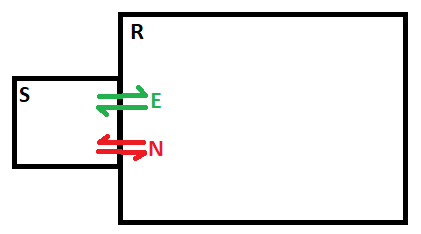
\includegraphics[width=0.25\textwidth]{graphs/GrandCan}
\end{wrapfigure}
In the grand canonical ensemble we allow for an exchange of energy and an exchange of particles then we have that the probability of a microstate is given by:
\[
p_s = \frac{e^{\frac{1}{k_B T}(\mu N_s - E_s)}}{\Theta}
\]
Where $\Theta$ is the grand canonical partition function which is defined as:
\[
\Theta(\mu, V, T) = \sum_{\text{microstates } s} e^{\frac{1}{k_B T}(\mu N_s - E_s)}
\]
An example of a system that could be described by the grand canonical ensemble is a room at constant humidity.  Then the chemical potential of water, the temperature and the volume are being kept fixed but everything else is allowed to change. Another way of writing the grand canonical partition function is:
\[
\Theta = \sum_s e^{\frac{1}{k_B T}(\mu N_s - E_s)} = \sum_N \sum_{s(N)} e^{\frac{1}{k_B T}(\mu N_s - E_s)} = \sum_N e^\frac{\mu N}{k_B T} \underbrace{\sum_{s(N)} e^{- \frac{E_s}{k_B T}}}_{Z_N} = \sum_{N = 0}^{+\infty} e^{\beta \mu N} Z_N
\]

\section{Grand Potential.}
We define the grand potential as:
\[
\Omega = -k_B T \log \Theta
\]
What we will know show is that $\Omega = F - \mu N = - p V$.
\subsubsection{Expression of $\Omega$.}
From the probability of a microstate we get that:
\[
p_N = \frac{e^{\beta \mu N} Z_N}{\Theta} \text{ and normalization immediately gives } \sum_{N = 1}^{+\infty} p_N = 1 \Leftrightarrow \Theta = \sum_{N = 1}^{+\infty} e^{\beta \mu N} Z_N
\]
We can see immediately that $p_N$ is very spiked in its average value, i.e $\Delta N \ll \bar{E}$. Then as done previously we use the method of steepest descent. First we re-write:
\[
\Theta = \sum_N e^{\beta \mu N} Z_N = \sum_N e^{\beta (\mu N - F_N)}
\]
Then we get that:
\[
\Theta = \int \dd N e^{\beta (\mu N - F_N)}
\]
The maximum of the exponent is given by:
\[
\pdv{}{N} (\mu N - F_N) = 0 \Leftrightarrow \mu = \pdv{F}{N}\Bigg|_{N^*}
\]
And we write:
\[
\mu N - F_N \approx \mu N^* - F_{N^*} + \cancelto{0}{\pdv{}{N} \left(\mu N - F_N\right) \Bigg|_{N^*}}(N - N^*) + \frac{1}{2} \pdv[2]{}{N}\left(\mu N - F_N\right) \Bigg|_{N^*}(N-N^*)^2
\]
Then plugging this back in the integral we have:
\[
\Theta \approx \int\dd N e^{\beta (\mu N^* - F_{N^*})} e^{\frac{\beta}{2}\pdv[2]{}{N} \left(\mu N - F_N\right)\big|_{N^*} (N - N^*)^2} = e^{\beta(\mu N^* - F_{N^*})} \underbrace{\sqrt{\frac{2\pi k_B T}{-\pdv[2]{}{N} \left(\mu N - F_N\right)\Big|_{N^*}}}}_{\sim \sqrt{N}}
\]
So we get that:
\[
\Omega = - k_B T \log \Theta  \approx F - \mu N
\]
Then the Legendre transformation of the above equation gives:
\[
F = E - TS
\]
\subsubsection{Relation of Gibbs-Duhem.}
The relation of Gibbs-Duhem says that $\mu, P, T$ are not independent. We already saw that:
\[
\dd F = - S \dd T - P \dd V + \mu \dd N, \quad \mu = \pdv{F}{N}\Bigg|_{T,V}, \quad P = -\pdv{F}{V}\Bigg|_{T,N}
\]
Since $F$ is an extensive variable we know that we can write is as:
\[
F(N,V,T) = Vf(\frac{N}{V}, T) = V f(\rho, T)
\]
Then:
\[
\mu = \pdv{F}{N}\Bigg|_{V,T} = V\frac{1}{V}\pdv{f}{\rho}\Bigg|_T = \pdv{f}{\rho}\Bigg|_T
\]
And similarly:
\[
P = - \pdv{F}{V}\Bigg|_{N,T} = -\pdv{}{V}\left[V f(\frac{N}{V}, T\right] = -f(\rho, T) - V \pdv{}{V} f(\frac{N}{V}, T)\Bigg|_{T, N} = -f - V \pdv{}{\rho} f(\rho, T)\Bigg|_T \pdv{\rho}{V} \Bigg|_T = -f + \rho \pdv{f}{\rho}\Bigg|_T
\]
So we can re-write this was:
\[
P = - f + \mu \rho \text{ therefore } PV = -F + \mu N
\]
Therefore going back to our previous result we get that:
\[
\Omega F - \mu N = - pV
\]
We now introduce the free enthalphy which is given by:
\[
G = F + PV = \mu N \quad \text{ so } \quad \mu = \frac{G}{N}
\]

\subsubsection{Differential version of Gibbs-Duhem.}
The simplest way of writing the Gibbs-Duhem in differential form is from:
\[
\dd F = - S\dd T - P\dd V + \mu \dd N
\]
We do a Legendre transformation to get:
\[
\dd G = - S\dd T + V \dd \rho + \mu \dd N \text{ and we have } \dd G = \dd (\mu N) = N \dd \mu + \mu \dd N
\]
So finally we get the following relation:
\[
N \dd \mu = - S \dd T + V \dd P
\]

\subsubsection{Average number of particles.}
With $T$ fixed the previous equation can be written as:
\[
\bar{N} = V \pdv{P}{\mu} \Bigg|_T = - \pdv{\Omega}{\mu}\Bigg|_{T, V}
\]

\section{Alternative approach.}
[...]

\section{Fluctuations and statistics.}
We showed previously that:
\[
p_N \approx \frac{1}{\Theta} \exp[\beta(\mu N^* - F_{N^*})] \exp[\frac{1}{2k_B T} \pdv[2]{}{N} \left(\mu N- F_N\right)\Bigg|_{N^*} (N - N^*)^2]
\]
From this we can deduce that:
\[
\langle (N - N^*)^2 \rangle = \frac{k_B T}{- \pdv[2]{}{N} \left(\mu N - F_N\right)\Big|_{N^*}}
\]
And we can re-write:
\[
-\pdv[2]{}{N}(\mu N - F_N) = \pdv[2]{F_N}{N}\Bigg|_{T, V} = \pdv{}{N} \mu \Bigg|_{T, V} \text{ with in the last equality } \mu = \pdv{F}{N}
\]
It can seem shocking to consider $\mu$ fixed at the start then we derive it, but the rigorous explanation of why this work is out of the scope of this text. Anyhow, with $T$ fixed we can write:
\[
N \dd \mu = V \dd P \Rightarrow \pdv{\mu}{N}\Bigg|_T = \frac{V}{N} \pdv{P}{N}\Bigg|_T \text{ then } \pdv[2]{F}{N} = \pdv{\mu}{N}|_{T,V} = \frac{V}{N} \pdv{P}{N}\Bigg|_T
\]
We then define the compressibility factor as:
\[
\chi_T = \frac{1}{V} \pdv{V}{P}\Bigg|_T
\]
Then:
\[
\pdv{P}{N} = \pdv{P}{\rho} \pdv{\rho}{N} = \frac{1}{V} \pdv{P}{\rho} \text{ and } \pdv{P}{V} = \pdv{P}{\rho} \pdv{\rho}{V} = -\frac{N}{V^2} \pdv{P}{\rho}
\]
So we have:
\[
\pdv{P}{N} = \frac{1}{V} \frac{-V^2}{N} \pdv{P}{V} = -\frac{V}{N}\pdv{P}{V} = \frac{1}{N \chi_T}
\]
So we deduce that:
\[
\pdv[2]{F}{N}\Bigg|_{T, V} = \frac{V}{N} \pdv{P}{N}\Bigg|_{T} = \frac{V}{N^2 \chi_T}
\]
So we can re-write our result above as:
\[
\langle (N - N^*)^2 \rangle = N \rho \chi_T k_B T
\]
\begin{wrapfigure}{r}{0.25\textwidth}
    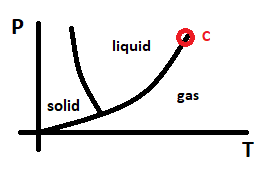
\includegraphics[width=0.25\textwidth]{graphs/critpoint}
\end{wrapfigure}
This is a main result that contains a lot of physics. First of all you can note that $\Delta N = \sqrt{\langle (N - N^*)^2 \rangle} \sim \sqrt{N}$ so that $\frac{\Delta N}{N} \sim \frac{1}{\sqrt{N}} \rightarrow 0$. We also get from observing the signs of the other terms that $\chi_T$ must be positive. This is what is called a condition of stability, it can happen that some states violate this condition but this will give rise to some fast changing out of equilibrium behaviors. Furthermore, if we look at a system close to the critical point where the transition in between liquid and gas stops (meaning that we cannot really differentiate our system as a liquid or a solid) so $\pdv{P}{V} \stackrel{(C)}{\rightarrow} 0$ so $\chi_T \stackrel{(C)}{\rightarrow} \infty$ therefore:
\[
\langle (N - N^*)^2 \rangle \stackrel{(C)}{\rightarrow} \infty
\]
So we see that the fluctuations diverge at a critical point.
\section{Alternative Approach (again).}
We saw that we can write:
\[
p_N = \frac{e^{\beta \mu N}}{\Theta} \text{ and we know that } \bar{N} = \langle N \rangle = \sum_N N p_N = \sum_N N \frac{e^{\beta(\mu N - F_N)}}{\Theta}
\]
So we can re-write:
\[
\bar{N} = \frac{1}{\beta \Theta} \pdv{}{\mu} \underbrace{\sum_N e^{\beta(\mu N - F_N)}}_\Theta = \frac{k_B T}{\Theta} \pdv{\Theta}{\mu} = k_B T \pdv{}{\mu} \log \Theta \text{ so } \bar{N} = - \pdv{}{\mu} \Omega \text{ where } \Omega = - k_B T \log \Omega
\]
Similarly we have that:
\[
\langle N^2 \rangle = \sum_N N^2 p_N = \frac{1}{\beta^2 \Theta} \pdv[2]{}{\mu} \Theta
\]
So we get that:
\[
\langle (N - N^*)^2 \rangle = \langle N^2 \rangle - \langle N \rangle^2 = (kT)^2 \left[ \frac{1}{\Theta} \pdv[2]{\Theta}{\mu} - \frac{1}{\Theta^2} \left(\pdv{\theta}{\mu}\right)^2 \right] = (k_B T)^2 \pdv{}{\mu} \left(\frac{1}{\Theta} \pdv{\Theta}{\mu}\right) = k_B T \pdv[2]{}{\mu} \Omega = k_B T \pdv{\bar{N}}{\mu}
\]

\section{Independent systems and factoring.}
[...]
\section{The perfect gas.}
In a system with no interaction we have:
\[
\Theta = \sum_s e^{\frac{\mu N_s}{k_B T} - \frac{E_s}{k_B T}} = \sum_N e^{\beta \mu N} Z_N
\]
We already calculated $Z_N$ for the perfect gas so we know:
\[
Z_N = \frac{1}{N!}\left(\frac{V}{\lambda^3}\right)^N \quad \text{ where } \quad \lambda = \sqrt{\frac{h^2}{2\pi m k_B T}}
\]
So we get that:
\[
\Theta = \sum_N e^{\beta \mu N} \cdot \frac{1}{N!} \left(\frac{V}{\lambda^3}\right)^N = \sum_N = \frac{1}{N!}\left(\frac{V e^{\beta \mu}}{\lambda^3}\right)^N = \exp(\frac{V e^{\beta \mu}}{\lambda^3})
\]
Which gives:
\[
\Omega = - k_B T \log \Theta = - k_B T \frac{V}{\lambda^3} e^{\beta\mu}
\]

\subsubsection{Pressure.}
We know that $\Omega = - PV$ so we get immediately that:
\[
P(\mu, T) = \frac{k_B T}{\lambda^3} e^{\beta \mu}
\]

\subsubsection{Number of particles.}
We have that:
\[
N = - \pdv{\Omega}{\mu} = \frac{V}{\lambda^3} e^{\beta \mu}
\]
So:
\[
\rho(T, \mu) = \frac{N}{V} = \frac{e^{\beta\mu}}{\lambda^3}
\]
Note that we obtain results that are completely equivalent to all the results obtained in the canonical ensemble.

\section{Example: Absorption on a surface.}
\begin{wrapfigure}{r}{0.25\textwidth}
    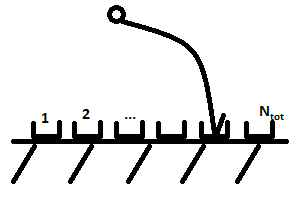
\includegraphics[width=0.25\textwidth]{graphs/absorbsurface}
\end{wrapfigure}
We introduce $N_{tot}$ variables $n_i$ which will be equal to 1 if the exist a particle in the box $i$ and 0 otherwise. Now for a given microstate $s$ we have that:
\[
E_s = \sum_i n_i \epsilon_0, \quad \text{ and } \quad N_s = \sum_i n_i
\]
Now we have two equivalent mathematical descriptions of the system:
\[
\Theta = \sum_{s} e^{\beta(\mu N_s - E_s)} \quad \text{ and } \quad \sum_N e^{\beta \mu N} Z_N
\]
We also introduce the fraction of occupied sites variable: $\frac{\bar{N_s}}{N_\text{tot}} = \Phi$. Then using the first description we have that:
\[
\Theta = \sum_s e^{\beta(\mu N_s - E_s)} = \sum_{\bigotimes_{i} \{s_i\} } e^{\beta \mu (\sum_i n_i - \sum_i n_i \epsilon_0)} = \sum_{\bigotimes_i \{s_i\}} \prod e^{\beta(\mu - \epsilon_0)n_i}
\]
So we get that:
\[
\Theta = \prod_i \sum_{n_i} e^{\beta(\mu - \epsilon_0)n_i} = \prod_i (1 + e^{\beta(\mu - \epsilon_0)}
\]
So in conclusion we have:
\[
\Theta = (1 + e^{\beta(\mu - \epsilon_0)})^{N_\text{tot}}
\]
Now if we use the second mathematical description we have that:
\[
\Theta = \sum_N e^{\beta \mu N} Z_N
\]
And by definition we have:
\[
Z_N = \sum_{s(N)} e^{-\beta E_s} = e^{-\beta N \epsilon_0} \cdot \# \text{ number of ways to get N particles}
\]
As always we have:
\[
\# \text{ nb of ways} = \begin{pmatrix}
N_\text{tot}\\N
\end{pmatrix}
= \frac{N_\text{tot}!}{N! (N_\text{tot} - N)!}
\]
So we have:
\[
\Theta = \sum_{N} \begin{pmatrix}
N_\text{tot}\\ N
\end{pmatrix}
e^{\beta(\mu - \epsilon_0)N} (1^{N_\text{tot} - N}) = \left(1 + e^{\beta(\mu - \epsilon_0)}\right)^{N_\text{tot}}
\]
So we indeed get the same result. Note that the second method is easier so long as we know the expression of $Z_N$ but since we usually use the grand canonical ensemble because we are unable to determine $Z_N$ in practice we will probably use the first method most of the time. From this we can deduce that:
\[
\bar{N} = - \pdv{\Omega}{\mu} = N_\text{tot} k_B T \pdv{}{\mu} \log(1 + e^{\beta(\mu - \epsilon_0})
\]
And also:
\[
\Phi = \frac{\bar{N}}{N_\text{tot}} = k_B T \frac{\beta e^{\beta(\mu - \epsilon_0)}}{1 + e^{\beta(\mu - \epsilon_0)}} = \frac{1}{1 + e^{\beta(\epsilon_0 - \mu)}}
\]
\begin{center}
	    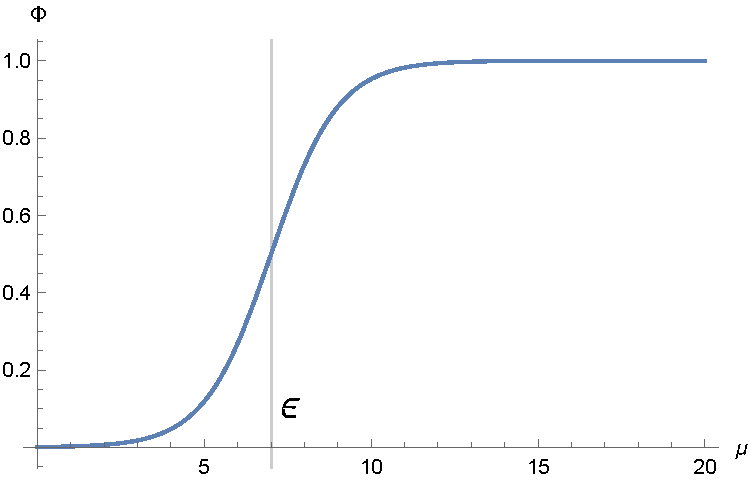
\includegraphics[width=0.5\textwidth]{graphs/plot_surface}
\end{center}

\section{Conclusion on ensembles.}
A good way to summarize what we saw with the different ensembles is with a table:
\begin{center}
\begin{tabular}{|c|c|c|c|}
\hline
Conditions & Ensemble & Partition function & Potential\\
\hline
$N, V, E$ & Micro Canonical & $\Omega = \sum_s \delta_{E_s, E} = \frac{1}{N!}\frac{1}{h^{3N}}\int_{E \leq \mathcal{H(\Gamma} \leq E + \Delta E} \dd \Gamma$ & $S = k_B \log \Omega = S(E, V, N)$\\
\hline
$N,V,T$ & Canonical & $ Z = \sum_s \exp(-\frac{E_s}{k_B T})$ & $ F = - k_B T \log Z = F(N, V, T) = E - TS$\\
\hline
$\mu, V, T$ & Grand Canonical & $\Theta = \sum_s \exp(\frac{\mu N_s - E_s}{k_B T})$ & $\Omega = -k_B T \log \Theta = \Omega(\mu, V, T) = F - \mu N = - P(\mu, T)V$\\
\hline
\end{tabular}
\end{center}
Note that every time we did the steepest descent method we implicitly wrote the following:
\[
F = \min_E \left( E - T S(E, V, N)\right),\quad F = \min_N \left(F(N,V,T) - \mu N\right), \quad G = \min_V \left( F(N,V,T) + PV\right)
\]
Other ensembles that we have not seen are the isobaric ensemble $(N, P, T)$, which has $p_s = \frac{1}{Y} e^{- \left(\frac{E_s}{k_B T} + \frac{P V_s}{k_B T}\right)}$. We also have $Y = \sum_s e^{-\frac{E_s + P V_s}{k_B T}} = \sum_V e^{-\frac{P V}{k_B T}} Z(N, V, T)$. And the potential is given by: $G = -k_B T \log Y= F + PV = \min_V (F(N, V, T) + PV)$. Furthermore remember that the Gibbs Duhem equation tells you that $F + PV = \mu N$. So we can also write: $G = \sum_{\text{species } i} \mu_i N_i$.

\chapter{Ideal systems and entropic forces.}
A good example of an ideal system is the ideal polymer that we have already treated previously. We have shown that if we pulled with a force $F$ on a polymer that had an extension of $\Delta x$ from its origin then we would get that:
\[
F = - K \Delta X, \quad \text{ with } K = \frac{k_B T}{R g^2} = \frac{k_B T}{N a^2}
\]
This is a good example of an entropic force. The idea behind entropic forces is that a system will always want to go to its most stable state. Therefore when we apply a constraint to the system that forces it out of optimum the system will resist with what is called an entropic force.

\section{Osmosis.}
\begin{wrapfigure}{r}{0.25\textwidth}
    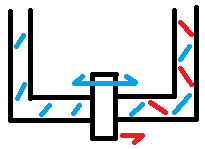
\includegraphics[width=0.25\textwidth]{graphs/Osmosis}
\end{wrapfigure}
Osmosis is striking because of its simplicity, subtlety and consequences. A simple system that shows it in action is the following. We take a tube of water separated on both sides by a filter that lets water pass but not salt and we add salt to the right of the tube. Then we will see that the water on the left will start going to the right side trying to balance the concentration on both sides in order to reach equilibrium. To stop this flux we could add a pump to the right hand side that would add a pressure of $\Delta \Pi = k_B T \Delta C_{\text{solution}}$ this is called the Vant Hoff formula. So we have a direct expression of the pressure due to the osmotic force. To give an idea of the orders of magnitude, if we have 1 mol of salt on the right and 0 on the left we get that $\Delta \Pi = 48 \text{bar}$. We will now prove this phenomenon and more specifically the Vant Hoff formula, using statistical physics. We assume that we are using ideal molecules which water is not, but we will see that it works nonetheless. So we take: $N_1$ molecules 1 and $N_2$ molecules 2 which are without interaction. For now we fix the the volume and the temperature. Since the two systems are independent the partition function is simply going to be given by the product, of the two partition functions. So we have:
\[
Z(N_1, N_2, V, T) = \frac{1}{N!}\left(\frac{V}{\lambda^3_T}\right)^{N_1} \frac{1}{N_2 !} \left( \frac{V}{\lambda^3_T}\right)^{N_2} = \frac{1}{N!}\left(\frac{V}{\lambda^3_T}\right)^N\frac{N!}{N_1 ! N_2 !} = Z_{\text{id}}(N, V, T) \cdot Z_\text{mix}(N_1, N_2)
\]
Where we have:
\[
Z_\text{id} = \frac{1}{N!} \left(\frac{V}{\lambda^3_T}\right)^N, \quad \text{ and } Z_\text{mix} = \frac{N!}{N_1!N_2!} = \begin{pmatrix}N\\N_1\end{pmatrix}
\]
So if we compute the potential we get that:
\[
F(N_1, N_2, V, T) = F_\text{id}(N, V, T) + F_\text{mix}(N_1, N_2, T)
\]
Where we have that:
\[
F_\text{id}(N, V, T) = - k_B T \log Z_\text{id} = - k_B T \log(\frac{1}{N!} \left(\frac{V}{\lambda^3_T}\right)^N), \text{ and } F_\text{mix}(N_1, N_2, T) = - k_B T \log Z_\text{mix} = -k_B T \log(\frac{N!}{N_1!N_2!})
\]
Then using the Stirling formula we get that:
\[
F_\text{mix}(N_1, N_2, T) = -k_B T \left( N\log N - N - N_1 \log N_1 + N_1 - N_2 \log N_2 + N_2 \right) = k_B T N (x_1 \log x_1 + x_2 \log x_2) 
\]
Where:
\[
x_i = \frac{N_i}{N_1 + N_2} \quad \text{ and } \quad x_1 + x_2 = 1
\]
We intuited before that the force comes from the system trying to stabilize the chemical potential, so that is what we want to compute now. We want to compute $\mu (T, P, x_1)$, which means that we have to pass from $V$ to $P$. To do so we use Gibbs-Free energy which is defined as: $G = \min_V (F(N_1, N_2, V, T) + PV)$. So we are looking for the volume for which $ \pdv{F}{V} + P = 0$. Since $F_\text{mix}$ is independent of $V$ we can write:
\[
\pdv{F_\text{id} + F_\text{mix}}{V} = \pdv{F_\text{id}}{V} = - P \Rightarrow \frac{k_B T}{V}N = P \Rightarrow V = \frac{N k_B T}{P}
\]
Then we write:
\[
G = F_\text{id}(N_1, N_2, V = \frac{N K_B T}{P}, T) + P \frac{N k_B T}{P} + F_\text{mix}(N_1, N_2, T) = \underbrace{Nk_B T \log (\frac{P}{k_B T} \lambda_T)}_{G_0 (T, P, N)} + Nk_B T (x_1 \log x_1 + x_2 \log x_2)
\]
Here we supposed that the two systems were ideal but more generally we will always have that:
\[
G(T, P, N_1, N_2) = G_0 (T, P, N) + G_\text{mix} (N_1, N_2, T)
\]
Now to make the link with our initial problem we write $N_1 = N_S$ the number of molecules of the solution and $N_1 = N_w$ the number of molecules of water. We further assume that $N_s \ll N_w$. Now we try to compute $\mu_w(T, P, x_s) = \pdv{G}{N_w}\Big|_{N_s, T, P}$. First we use our assumption of $N_s \ll N_w$ to simplify $G$:
\[
G = G_0(T, P, N_s + N_w) + k_B T \left(N_s \log \frac{N_s}{N_s + N_w} + N_w \log \frac{N_w}{N_s + N_w}\right) \approx G_0(T, P, N_s + N_w) + k_B T \left( N_s \log \frac{N_s}{N_w} - N_s \right)
\]
Which gives:
\[
\mu_w(T, P, x_s) = \pdv{G}{N_w}\Bigg|_{N_s, T, P} = \mu_0(T, P) - k_B T \frac{N_s}{N_w} \approx \mu_0 (T, P) - k_B T x_s
\]
We now consider the system where we apply a pressure on the right hand side to stop this osmotic flow. Then on the left of the filter we have $\mu_w(T, P, x_s = 0)$ and on the right we have $\mu_w(T, P + \Delta Pi, x_s)$ and equilbrium dictates that:
\[
\mu_w(T, P, x_s = 0) = \mu_w(T, P + \Delta Pi, x_s) \Leftrightarrow \mu_0 (T, P) = \mu_0 (T, P + \Delta \Pi) - k_B T x_s
\]
Now if we assume that $\Delta \Pi$ is small we can re-write as:
\[
\mu_w(T, P + \Delta \Pi) - \mu_w(T, P) = \pdv{\mu_w}{P} \Delta\Pi
\]
And using the Gibbs-Duheim equation we have that $N\dd\mu = V \dd P$ so that $\pdv{\mu}{P} = \frac{V}{N_w}$. Now plugging this in we get that:
\[
\Delta \Pi = k_B T \frac{N_s}{N_w} = k_B T C_s
\]
Which concludes the proof.

\subsubsection{Alternative demonstration.}
Another way to approach the problem is to make a force balance. One thing to note is that the filter, though crucial to the problem, has absolutely no influence on the final results. So we decide to replace the filter by a simple potential barrier: $\mathcal{U}_s(x)$ which does not act on water and is very peaked at 0 with $\max \mathcal{U}_s \gg k_B T$. Now if we write Boltzmann's law for particles in presence of a potential we have:
\[
c_s(x) = \underbrace{c_s}_{x = +\infty} \exp(-\frac{\mathcal{U}_s (x)}{k_B T})
\]
The question now is what is the force due to the filter on the fluid. To compute it we decompose it as such:
\[
\frac{F}{A} = \sum_\text{particles} \underbrace{f_i}_\text{force on a molecule of salt} = \sum_\text{salt} \left(- \pdv{\mathcal{U}_s}{x}\right)
\]
Which we can re-write as:
\[
\frac{F}{A} = \int \dd x c_s(x)x \left(- \pdv{\mathcal{U}_s}{x}\right) = \int \dd x c_s e^{-\frac{\mathcal{U}_s(x)}{k_B T}} (- \partial_x \mathcal{U}_s) = \int \dd x c_s k_B T \partial_x e^{-\frac{\mathcal{U}_s(x)}{k_B T}} = k_B T c_s \left(\underbrace{e^{-\frac{\mathcal{U}_s(\infty)}{k_B T}}}_{1} - \underbrace{e^{-\frac{\mathcal{U}_s(0)}{k_B T}}}_{0}\right)
\]
So we finally get that:
\[
\frac{F}{A} = \Delta \Pi = k_B T c_s
\]
We see here two different ways of understanding the osmotic force. The first is to consider it as a force that tries to bring back the system to equilibrium and the second is simply the mechanical force that filter itself exercises on the system to push back the molecules of salt.

\section{Forces and depletion.}
We now consider a system that contains "big particles" called colloids and "small particles" called polymers. Usually these particles are in a solvent but since it has no role in the problem we forget about it. We call $R$ the radius of the colloids and $R_g$ the radius of the polymers ($R \gg R_g$). Now if we consider a single colloid we see that the excluded volume for the polymer is going to be $V_\text{exl}^0 = \frac{\pi}{6} \left(2(R + R_g)\right)^3 = \frac{\pi}{6} D^3$. Now if we consider two colloids far apart we simply get again that:
\[
V_\text{accessible} = V - 2 V_\text{excluded}^0
\]
But when we take two colloids close together the situation becomes more complicated because there is an overlap in the forbidden areas induces by each colloid. So we get that $V_\text{excl} < 2 V_\text{excl}^0$. Now to compute the area we have to do simple geometry. If we consider two colloids whose borders are separated by a distance $h$. Then we get that $\cos \theta = \frac{R + h/2}{R+ R_g}$. Which then gives that:
\[
V_\text{excl} = 2 (\frac{\pi}{6}D^3 - V_\text{overlap}) = 2 (\frac{\pi}{6}D^3 - \frac{\pi}{3} (\underbrace{(R + R_g) - (R + \frac{h}{2})}_{d})^2(3(R+ R_g) - d)
\]
Which re-written more cleanly gives:
\[
V_\text{excl} = \frac{\pi D^3}{6}\left( 1 + \frac{3}{2} \frac{r}{D} - \frac{1}{2} \left(\frac{r}{D}\right)^2\right), \quad \text{ with } r = 2R + h \text{ and } D = 2(R+R_g)
\]
The question we now want to answer is what is the force in between the 2 colloids. We assume the colloids fixed and we study the phase space of the polymers. We have that:
\[
V_\text{accesible} = V_\text{acc} = V - V_\text{excl} (r)
\]
So the partition function is:
\[
Z = \frac{1}{N!}\left(\frac{V - V_\text{excl}(r)}{\lambda_T^3}\right)^{N_p}
\]
The potential is given by $F = -k_B T \log Z$ and the force is:
\[
\mathcal{F} = -\pdv{F}{r} = k_B T N_p \pdv{}{r} \log(V - V_\text{excl}(r)) = k_B T \frac{N_p}{V - V_\text{excl}} \pdv{}{r} V_\text{excl}(r)
\]
If we write $c_p = \frac{N_p}{V - V_\text{excl}}$ we get:
\[
\mathcal{F} = k_B T c_p \left(-\pdv{V_\text{excl}}{r}\right)
\]
Now we saw earlier that for $r > D$ we have that $V_\text{excl} = 2V_\text{excl}^0$ which is a constant and below $D$ the exluded volume will decrease (i.e. the function is increasing). Therefore we get that the force is going to be 0 when $r > D$ and negative (i.e. attractive) when $r < D$. The physical understanding of this is that when the colloids are closer together the phase space of the polymers becomes bigger and therefore the the entropy increases. So we have simply another example of an entropic force.

\section{Miscellaneous systems.}
\section{Forces induced by fluctuations.}
There are three main configurations: Casimir - De Gennes Fisher - Helfrisch, we will focus more on the Helfrisch.
\subsubsection{Casimir}
The Casimir forces caracterize the fluctuations of, for example, a magnetic field in between two charged plates separated by $D$ in void. Then we get that the field will be expressed in modes given by the following equation; and an attractive force due to the fluctuations will appear:
\[
k_n = \frac{2\pi}{D} n \quad \text{ furthemore } \frac{F}{A} = \frac{-\pi^2}{240}\frac{\hbar c}{D^4}
\]
\subsubsection{'Critical' forces - De Genes, Fisher.}
For more detail one can go see C.R.A.S of 1978 (Compte Rendu de l'Academie des Sciences) or C. Bechinger Nature 2007. This configuration studies systems that are close to the critical point of transition in between liquid and gas. So considering the same system as above but immersed in a fluid at $(C)$ we get:
\[
\frac{F}{A} \sim - \frac{kT}{D^2}
\]
\subsubsection{Forces Helfrisch.}
Helfrisch studies a superposition of membranes separated by $D$ then we see that a repulsive force appears, expressed as:
\[
\frac{F}{A} \propto \left(\frac{kT}{D}\right)^2
\]
The priniple is that an elastic membrane will be able to explore some configurations of its phase space thanks to the ambient temperature, having a characteristic height $\langle h^2 \rangle$. When we confine the membrane in a rectangle of height $D$, i.e. we apply a constraint, the membrane might be forced out of its average value and will have $\langle h^2 \rangle_\text{confined} \sim D^2 < \langle h^2 \rangle_\text{free}$, and therefore as we saw previously this will induce an entropic force that will tend to go back to equilibrium. So overall we expect to find a repulsive force in between the membranes.

\subsubsection{Simplified Model.}
Normally we should consider an elastic membrane but to simplify we will make an analogy to a 1D elastic string. [...] So we see that for an elastic string we get that:
\[
H = \underbrace{\sum_i \frac{1}{2} \tilde{k} (h_{i+1} - h_i)^2}_{\text{string energy}} + \underbrace{V(h)}_{\text{constaint}} \quad \text{ and we take } \quad V(h) = \sum_i \frac{1}{2} \tilde{K} h_i^2
\]
Now we will write $H(h_1, \cdots, h_N) = H(\{h\})$ where $\{h\}$ is a functional. We also say that the probability of finding a given state is:
\[
p(\{h\}) = p(h_1, \cdots, h_N) \propto \exp[-\frac{1}{k_B T} H(\{h\})]
\]
Then for any observable $A$ we get:
\[
\langle A \rangle = \frac{\int \dd h_1 \cdots \dd h_N A(\{h\}) \exp[-\frac{1}{k_B T}]}{\int \dd h_1, \cdots \dd h_N \exp[-\frac{1}{k_B T}]}
\]
And we also have:
\[
Z = \int \dd h_1 \cdots \dd h_N \exp[-\frac{1}{k_B T} H(\{h\})]
\]
Now we will first compute the $\langle h^2 \rangle$ and then we will compute the free energy $F = -k_B T \log Z$.
\subsubsection{Average extension.}
We have:
\[
\langle h^2 \rangle = \frac{1}{L} \int_0^L \dd x \langle h^2(x) \rangle
\]
Note also that passing from the continous model to the discrete one can be written as (where $a$ is the lattice size in the discrete case):
\[
H(\{h\}) = \sum_i \frac{1}{2}\tilde{k}(h_{i+1} - h_i)^2 + \frac{1}{2}\tilde{K} h_i^2 \quad \text{ and } \quad \sum_i = \int \frac{\dd x}{a}
\]
Then we get that:
\[
H(\{h\}) = \int_0^L \dd x \left[ \frac{1}{2} k (\grad h)^2 + \frac{1}{2} K h^2\right] \quad \text{ with } \grad = \dv{}{x}
\]
Now see that the difficulty comes from the interaction between nearest neighbors, but if we pass to the Fourier space the problem simplifies. As a general rule in such problems passing to the Fourier space separates the modes and allows for an easier treatment of the problem. From definition we have:
\[
p(\{h\}) = \frac{1}{Z} \exp[-\frac{1}{k_B T} \int \dd x \left(\frac{1}{2} k(\grad h)^2 + \frac{1}{2} K h^2\right)]
\]
Then remember the definition of the Fourier transforms:
\[
h_q = \int \dd x h(x) e^{iqx} \quad \text{ and } \quad h(x) = \int \frac{\dd q}{2 \pi} h_q e^{-iqx}
\]
We also have the Parceval theorem:
\[
\int \dd x f(x)^2 = \int \frac{\dd q}{2 \pi} |f_q|^2
\]
Furthermore when transforming the gradient we get $\grad \stackrel{\text{FT}}{\longrightarrow} - iq$ so overall:
\[
\int \dd x \pdv{h}{x} e^{iqx} \stackrel{\text{FT}}{\longrightarrow} -iq \int \dd x h e^{iqx} = -iq h_q
\]
So the whole integral simplifies to (making a FT and applying Parceval):
\[
\int \dd x \left(\frac{1}{2} k(\grad h)^2 + \frac{1}{2} K h^2\right)  = \int \frac{\dd q}{2 \pi} \frac{1}{2} (kq^2 + K) |h_q|^2
\]
So with a bit of computations we get that:
\[
\exp[-\frac{1}{k_B T} \int \dd x \left(\frac{1}{2} k(\grad h)^2 + \frac{1}{2} K h^2\right)] = \exp[-\frac{1}{k_B T}\underbrace{\int \frac{\dd q}{2\pi} \frac{1}{2} (kq^2 + K) |h_q|^2}_{\frac{1}{L}\sum_{\{q_n\}} \frac{1}{2} (kq^2 + K) |h_{q_n}|^2}]
\]
So finally we obtain:
\[
p(\{h\}) = \frac{1}{Z}\prod_{\{q_n\}} \exp[-\frac{1}{2k_B T L} (k q^2 + K) |h_{q_n}|^2]
\]
From here we can conclude that the $h_{q_n}$ variables are independent and quadratic. So we can use what we had previously computed for equipartition and we get:
\[
\frac{1}{2L} (kq_n^2 + K) \langle |h_{q_n}|^2 \rangle = \frac{1}{2} k_B T \cdot 2
\]
Note that we have a factor of 2 on the right because in reality $h_{q_n}$ is a complex variable so it has two degrees of freedom: its real and imaginary part. So finally we get:
\[
\langle |h_q|^2 \rangle = \frac{2 k_B T L}{k q^2 + K}
\]
Coming back to the original question we have:
\[
\langle h^2 \rangle = \frac{1}{L} \int_0^L \dd x \langle h(x)^2 \rangle = \frac{1}{L} \int_{-\infty}^{+\infty} \frac{\dd q}{2\pi} \langle |h_q|^2 \rangle = \frac{1}{L}\int \frac{\dd q}{2\pi}\frac{2 k_B T L}{kq^2 + K} = \frac{k_B T}{\pi} \int \dd q \frac{1}{kq^2 + K} = \frac{k_B T}{\pi K}\int  \sqrt{\frac{K}{k}} \frac{\dd u}{1 + u^2}
\]
So finally we get that:
\[
\langle h^2 \rangle = \frac{k_B T}{\sqrt{k K}}
\]
Note that the fluctuations of the membrane increase linearly with temperature, so it really can explore a vast amount of its phase space. In reality it is what we observe as well, membranes have very important fluctuations.
Note that we shifted slightly from the original problem. We considered a harmonic potential while in reality we wanted to model a potential well, but note that we said previously that $\langle h^2 \rangle = D^2$, so that making the analogy we assume that we can shift from one problem to the other by taking:
\[
\frac{k_B T}{\sqrt{k K}} = D^2 \Rightarrow K = \frac{1}{k}\left(\frac{k_B T}{D^2}\right)^2
\]
\subsubsection{Free Energy.}
Now we want to compute the free energy: $\mathcal{F}$, and more particularly $\Delta \mathcal{F} = \mathcal{F}(D) - \mathcal{F}(D \to \infty)$. We have:
\[
Z(\{h\}) = \int \dd h_1 \cdots \dd h_N \exp[\underbrace{-\frac{1}{k_B T} \sum_i \left( \frac{1}{2} \tilde{k}(h_{i+1}-h_i)^2 + \frac{1}{2}\tilde{K} h_i^2 \right)}_{= \mathbf{H}^T \mathbf{A} \mathbf{H}}]
\]  
Note that what is written inside the exponential could be written as a matrix product with a coupling matrix $A$ and solved in such way. But we will simplify it using the Fourier Transform:
\[
Z(\{h\}) = \int \dd h_1 \cdots \dd h_N \exp[ -\frac{1}{k_B T} \sum_{q_n} \frac{1}{2}(kq_n^2 + K)|h_{q_n}|^2 ] = \prod_{q_n} \underbrace{\int \dd h_{q_n} \exp[ -\frac{1}{2 k_B T} (kq_n^2 + K)|h_{q_n}|^2 ]}_{\frac{1}{2} \cdot 2 \quad \text{(Re and Im)}}
\]
So finally we get that:
\[
Z = \prod_{q_n} \left(\frac{2\pi k_B T}{k q_n^2 + K}\right)
\]
Note that mathematically what we are doing is simply to diagonalize the coupling matrix $A$, getting independent terms and then performing the integral. Here though we have a physical interpretation of what we are doing, which is to pass the the Fourier modes of the system which behave independently. Now to compute the free energy we have that:
\[
\mathcal{F}(K) = - k_B T \log Z = - k_B T \sum_{q_n} \log \frac{2 \pi k_B T}{k q_n^2 + K} = - k_B T L \int \frac{\dd q}{2\pi} \log \left(\frac{2\pi k_B T}{kq^2 + K}\right)
\]
Which gives:
\[
\Delta \mathcal{F} = \mathcal{F}(D) - \mathcal{F}(D \to \infty) = \mathcal{F}(K) - \mathcal{F}(K = 0) = - k_B T L \int \frac{\dd q}{2 \pi} \log(\frac{kq^2}{kq^2 + K})
\]
So we get that:
\[
\frac{\Delta \mathcal{F}}{L} = -k_B T \underbrace{\int \frac{\dd q}{2 \pi}}_{u = \sqrt{\frac{k}{K}}q} \log(1 + \frac{K}{kq^2}) = C k_B T \sqrt{\frac{K}{k}}
\]
Now using what we said previously: $\frac{k_B T}{\sqrt{k K}} = D^2$ we get that:
\[
\frac{\Delta \mathcal{F}}{L} = C \left(\frac{k_B T}{D}\right)^2 = \text{'Hellfrisch'}
\]
Note that this is not the full result since Hellfrisch really does the full computation considering an elastic membrane, but we still get all the basic physics involved from this result. Furthermore note that the force associated with this is given by:
\[
P(D) = - \pdv{\mathcal{F}}{V} = -\pdv{}{D} \left(\frac{\mathcal{F}}{\mathcal{A}}\right) = \frac{2 C (k_B T)^2}{k D^3}
\]

\chapter{Statistical ensembles and thermodynamics.}
Up to now we have introduced the basic tools of statistical physics. We have, from time to time, showed the link with thermodynamics but now we will make a sort of intermediary chapter that will resume all of the main thermodynamic principles from statistical physics. If you want more details on this Callen is a good reference.

\section{Back to thermodynamic principles.}
\subsection{Definitions.}
We start by a few definitions to set the vocabulary we are going to work with:
\begin{itemize}
\item \textbf{State variables}: variables which characterize the thermodynamic state of a system ($N, P, T, \mu, \cdots$). One of the big surprises of thermodynamics is that very few variables are required to describe very complex systems. This is due to the fact that the systems are very large and therefore can usually be considered as being only small variations away from its average values.
\item \textbf{Order parameters}: these are the parameters that 'quantify' the state of the system. So for example in spin system, i.e. a succession of up/down polarized dipoles, the mean value of the magnetic moments: $m$, is an order parameter. Since it will tell if the system is polarized ($m \neq 0$) or not ($m = 0$). Another example is the liquid/solid transition. If we define:
\[
\rho_G = \frac{1}{N}\sum_i e^{i \vec{G} \cdot \vec{r_i}}
\]
Where $\vec{G}$ is the vector of the reciprocal lattice of the solid (i.e. $\vec{r_i}\cdot \vec{G} = 2\pi k$), then $\rho_G$ is going to be 0 for a liquid and 1 for a solid. And for the liquid/gaz transition the density is an order parameter.
\item \textbf{State function}: a state function is a function of state variables.
\item \textbf{Reversible transformation}: A transformation that can be done both ways.
\end{itemize}

\subsection{Principles.}
\subsubsection{First Principle.}
The variation of energy of a system is the sum of the work and heat received:
\[
\dd E = \delta W + \delta Q \quad \text{ and } \quad \Delta E = W +Q
\]
From this we also deduce that $E$ is a state function: $E = E(S, V, N)$. Note also that we are going to use the banker's convention, i.e. what is coming in is positive and what is coming out is negative. SO $\delta Q > 0$ and $\delta W > 0$ is the quantity of received heat (resp. work) for the system.
\subsubsection{Second Principle.}
There exists a function $S$, entropy, function of the extensive parameters characterizing the macroscopic state, such that in all transformation towards an equilibrium state, in an isolated system, $\Delta S \geq 0$.\\
Another formulation of this principle is the following. The values taken by the extensive state parameters when the constraint is freed are those that maximize the entropy over all the constrained equilibrium states. Let us explicit what we mean by this. Let $X$ be a constraint, then $S = S(E,V,N,X)$. The second principle states that the equilibrium without constraint is defined as $\max_X S(X)$.\\
\subsubsection{Link with heat exchange.}
In a reversible transformation we have that:
\[
\dd S = \frac{\delta Q}{T}
\]
In an irreversible transformation we have that:
\[
\dd S > \frac{\delta Q}{T}
\]
Note that the second relation comes from the fact that if we consider a system $S$ in contact with a much larger system $R$, the whole being isolated. Then the huge system $R$ can be considered always at equilibrium and $\delta Q = T_0 \dd S_R$, and since the whole is isolated we get:
\[
\begin{cases}
\dd E_\text{tot} = \dd E_S + \dd E_R\\
\dd S_\text{tot} \geq 0
\end{cases}
\]
And:
\[
\dd S_\text{tot} = \dd S_s + \underbrace{\dd S_R}_{-\frac{\delta Q}{T_0}} \geq 0 \Rightarrow \dd S_s \geq \frac{\delta Q}{T_0}
\]

\subsection{Thermodynamic and thermic engines.}
A thermic engine is a system that exchanges work and heat in cycles. Note that engine respect some rules that follow from the thermodynamics principles, like the impossibility of perpetual motion of the second kind:
\begin{center}
A machine that does a cycle with only one source of heat cannot produce work.
\end{center}
\subsubsection{Proof}
The key to the proof is to notice that over a cycle:
\[
\begin{cases}
\Delta E = 0\\
\Delta S = 0
\end{cases}
\]
Since both $E$ and $S$ are state functions and since at the end of a cycle we come back to the initial state the difference will be null. We also have the following equations:
\[
\begin{cases}
\Delta E = Q + w = 0\\
0 = \Delta S \geq  \frac{Q}{T_0}
\end{cases} \Rightarrow Q \leq 0 \land W \geq 0
\]
So the system necessarily receives work and does not produce any. \\\\
Here the resolution was quite evident but we can easily go to very difficult problems around this question. A famous problem from Feinmann is the one where we consider a dented wheel with a ratchet stopping the anti-clockwise-rotations of the wheel and a weight on the left side of the wheel. Then if we allow the system to have thermic fluctuations then the wheel has thermic fluctuations and the ratchet allowing the system only to move on the right then we should lift the weight. Thermodynamics tells us that this is impossible but it can be quite hard to notice where we went wrong. The actual mistake is that statistical physics tells us that we need a balance of probability in our system which means that we have to consider the thermic fluctuations of the ratchet itself as well.

\subsubsection{Two heat sources engine.}
We now take an engine $M$ that takes $Q_1$ from a thermic bath $T_1$ and outputs $W$ and $Q_2$ to a thermic bath $T_2$. As before, we have:
\[
\begin{cases}
\Delta E = 0 = Q_1 - Q_2 - W\\
\Delta S = 0 \geq \frac{Q_1}{T_1} - \frac{Q_2}{T_2}
\end{cases}
\]
Now let's intrest ourselves to a special quantity, the efficiency: $\nu = \frac{W}{Q_1}$, then from our equations above we get that:
\[
\begin{cases}
Q_2 = Q_1 - W\\
\frac{Q_2}{T_2} \geq  \frac{Q_1}{T_1}
\end{cases}
\Rightarrow 1 - \nu \geq \frac{T_2}{T_1} \Rightarrow \nu \leq 1 - \frac{T_2}{T_1}
\]
So we see that we have an upper bound on efficiency, it is impossible to have a perfectly efficient engine. This concludes our short reminders on thermodynamics, but the reader is strongly invited to go and read more about it in the reference books cited at the end.

\section{Thermodynamics and ensembles.}
\subsection{Conclusion on the different ensembles.}
We have:
\begin{center}
\begin{tabular}{c | c | c |}
isolated system & $N, V, E$ & $S(E,V, N)$\\
\hline
fixed temperature system & $N, V, T$ & $F(N, V, T)$\\
\hline
$T, \mu$ fixed system & $\mu, V, T$ & $\Omega(\mu, V, T)$\\
\hline
$T, P$ fixed system & $N, P, T$ & $G(N, P, T)$\\
\hline
\end{tabular}
\end{center}
We also have the following equations:
\[
\begin{cases}
\dd E = T \dd S - P \dd V + \mu \dd N\\
\dd F = - S \dd T - P \dd V + \mu \dd N\\
\dd \Omega = - S \dd T - P \dd V - N \dd \mu\\
\dd G = - S \dd T + V \dd P + \mu \dd N
\end{cases}
\]
\subsection{Maxwell relations}
From the above we immediately get that:
\[
\begin{rcases}
P = - \pdv{F}{V} \Big|_{T, N}\\
\mu = \pdv{F}{N} \Big|_{V,T}
\end{rcases}
\quad \pdv{P}{N} \Bigg| = -\pdv[2]{F}{N}{V} = - \pdv[2]{F}{V}{N} = -\pdv{\mu}{N}
\]
So we have:
\[
\begin{rcases}
-S = \pdv{F}{T}\\
-P = \pdv{F}{V}
\end{rcases}\quad \pdv{S}{V} = - \pdv[2]{F}{T}{V} = -\pdv[2]{F}{V}{T} = \pdv{P}{T}
\]

\subsection{Equilibrium and release of constraints.}
We consider an isolated system that is under a constraint $X$. Remember that we stated previously that equilibrium was defined for:
\[
S_\text{eq} = \max_X \{S(X)\}
\]
Intuitively a way to understand this is to say that at equilibrium the system will be able to explore as much of it's phase space as possible therefore $S = k_B T \log \Omega$ will be maximal. To give an example we consider a system in contact with a thermostat at temperature $T_0$, we split the volume of our system $V$ in two volume $V_1,V_2$ and put a constraint on $V_1$. Then $Z$ will be a function of $V_1$ and we get:
\[
p(X_1 = V_1) = \frac{1}{Z} \sum_{\text{micro states } s_1, s_2} e^{-\beta E_{s_1}} e^{- \beta E_{s_2}} \delta_{X_{s_1} = X_1} \delta_{X_{S_2} = X_2} = \frac{Z_1(X_1)Z_2(X_2 = X_\text{tot} - X_1)}{Z_{1 \cup 2}}
\]
Where we use:
\[
\begin{cases}
Z_1(X_1) = e^{-\beta F(X_1)}\\
Z_2(X_2) = e^{-\beta F(X_2)}
\end{cases}
\]
So we get that:
\[
P(X_1) = \frac{1}{Z_\text{tot}} e^{-\beta F_\text{tot}(X_1)} \quad \text{ with } \quad F_\text{tot}(X_1) = F_1(X_1) + F_2(\underbrace{X_\text{tot} - X_1}_{X_2})
\]
\subsubsection{Consequences.}
The maximal probability is given for $F_\text{tot}(X_1)$ being minimal, and we have:
\[
\pdv{F_\text{tot}}{X_1} = 0 = \underbrace{\pdv{F_1}{X_1}}_{x_1} - \underbrace{\pdv{F_2}{X_2}}_{x_2}
\]
Where $x_i$ are the intensive parameters associated to $X_i$. Then we have $X_1 =V_1$ which gives $x_1 = -p_1$ and $p_1 = p_2$ which is our equilibrium condition.

\subsubsection{Example of Application.}
We consider a system in contact with a bath at $T, \mu$. Then we have $\Omega = \Omega(\mu, V, T)$. In practice now we could try and compute the partition function itself or we could consider the free energy and make some simplifications on the free energy. We know:
\[
\frac{F}{V} = f(\rho) \quad \text{ where } \quad \rho = \frac{N}{V}
\]
For an ideal system we have:
\[
f_\text{id}(\rho) = k_B T (\rho \log \rho \lambda_T - \rho)
\]
And more generally we have:
\[
f(\rho) = f_\text{id}(\rho) + f_\text{int}(\rho)
\]
For example, it is not uncommon to make an approximation on $f_\text{int}$ and take it to be: $f_\text{int}(\rho) = \frac{1}{2}B \rho^2$. Which is called a viriel development. Now if we define:
\[
\Omega = F - \mu N \quad \text{ we get that } \quad \Omega = \Omega(\rho, \mu, V, T) = \Omega(N, \mu, V, T)
\]
So we have on parameter too much, but this is a typical example of a constraint. When computing this we considered states that were only at a given $\rho$ and by the previous development we know that equilibrium will be given for $\min_N \Omega$. So we want:
\[
\pdv{\Omega}{N} = 0 \Rightarrow \pdv{f}{\rho}\Bigg|_\text{eq} = \mu 
\]
We also know that:
\[
\text{prob}(\{\rho\}) \propto e^{-\beta F(\rho)} = e^{-\beta V f(\rho)}
\]

\section{Stability conditions and fluctuations.}
We already said that at equilibrium $S$ must be maximal. This immediately induces that:
\[
\pdv{S}{X}\Bigg|_\text{eq} = 0 \quad \land \quad \pdv[2]{S}{X}\Bigg|_\text{eq} \leq 0
\]
Identically for $F$ we get that $F$ must be minimal therefore:
\[
\pdv{F}{X}\Bigg|_\text{eq} = 0 \quad \land \quad \pdv[2]{F}{X}\Bigg|_\text{eq} \geq 0
\]
From the properties of convex functions we also get that:
\[
2 F(\frac{N}{2}, \frac{V}{2}, T) = F(N, V, T) \leq F(\frac{N}{2} - n, \frac{V}{2} - v, T) + F(\frac{N}{2}+ n, \frac{V}{2} + v, T)
\]
Remark also that:
\[
\pdv[2]{F}{T} \leq 0 \quad \text{ idem for } G, H, P, \cdots
\]
\subsubsection{Example.}
An example is the compressibility factor:
\[
\chi_T = -\frac{1}{V} \pdv{V}{P} \Bigg|_T \propto \left( \pdv[2]{F}{V}\Bigg|_T \right)^{-1} \geq 0 \quad \text{ and } \quad P = -\pdv{F}{V}
\]
Note that this is compatible with:
\[
0 \leq \langle\Delta N^2 \rangle = N k_B T \rho \chi_T
\]

\section{Thermodynamics and change of phase.}
\begin{wrapfigure}{r}{0.25\textwidth}
    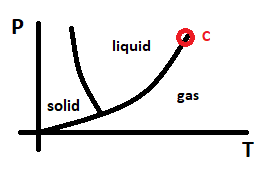
\includegraphics[width=0.25\textwidth]{graphs/critpoint}
\end{wrapfigure}
We are now going to interest ourselves with a system that starts in a point $A$ in the gas phase and end at $B$ in a liquid phase. The questions we want to answer are what are the characteristics of this transition and what is the signature of this signature on the thermic potential.

\subsection{Order parameters and transitions orders.}
We have already discussed order parameters. To refresh your memory we will give 2 examples. When we want to differentiate liquid from gas we consider $\rho$ as an order parameter. If we consider a spin polarity we would consider the mean polarity: $m = \frac{1}{N}\sum_i S_i$.

\subsubsection{2 Behaviors.}
We have 2 possible transition types. The first is when $\Phi$ (our order parameter) makes a discontinuous jump for some critical values of $T, \mu, P$. This is a transition of the first order. The second is $\Phi$ starting at a non-negative value and decreasing to 0, and when reaching 0 stopping there. An example of this is the spin transition, here $\Phi$ is continuous. This is a second order transition.

\subsubsection{1st Order Transition.}
Note that the discontinuity in the order parameter will induce a discontinuity or even a divergence in the first derivatives of the thermic potentials like $N = -\pdv{\Omega}{\mu}\Bigg|_{T,V}$.

\subsubsection{2nd Order Transition.}
For the 2nd Order transition we get the same behavior but now for the second derivative of the thermic potentials, which become discontinuous or even divergent.

\subsubsection{Example 1.}
We want to study the liquid-gas transition. We know that $\rho$ is going to be discontinuous at the transition. To do so we work with $(\mu, V, T)$ fixed. We will call the transition point, the coexistence point or the saturation point. At the transition we get that:
\[
P_l = P_g \quad \text{ and } \quad \mu_l = \mu_g
\]
Because of the transition $\Omega$ has a different behavior for $\mu < \mu_\text{coex}$ and $\mu > \mu_\text{coex}$. Its as if we have two functions, one for the liquid phase and one for the gaseous phase. And the system will keep only the minimal value (for $\Omega$, so the maximal value for $P$) of the two. We therefore get a singularity at the crossing point of the two functions.

\subsubsection{Latent Heat.}
Note that at the transition the entropy is also discontinous:
\[
S = - \pdv{\Omega}{T}\Bigg|_{V, \mu}
\]
So we introduce a new variable to characterize this jump called the latent heat of the transition:
\[
L_{l\leftrightarrow g} = T (S_\text{gas} - S_\text{liquid})
\]

\subsubsection{Clapeyron Relation.}
If we take two pairs of points symmetric with respect to the transition curve on the $P,T$ graph we get that $\mu_A = \mu_B$ and $\mu_{A'} = \mu_{B'}$. Note that we also have the Gibbs-Duhem relation:
\[
\Rightarrow \dd \mu = \frac{V}{N} \dd P - \frac{S}{N}\dd T
\]
We know apply this to both sides of the curve (gaseous and liquid phase):
\[
\dd \mu = \mu_{A'} - \mu_A = \frac{V_g}{N} \dd P - \frac{S_g}{N} \dd T \quad \text{ and } \quad \dd \mu = \mu_{B'} - \mu_{B} = \frac{V_l}{N} \dd P - \frac{S_l}{N}\dd T
\]
But from what we said previously we need these two to be equal, which gives:
\[
v_g \dd P - s_g \dd T = v_l \dd P - s_l \dd T
\]
Where we use $v = \frac{V}{N}$ and $s = \frac{S}{N}$, then one the transition curve:
\[
\dv{P}{T} = \frac{s_g - s_l}{v_g - v_l} = \frac{T \l_{g\leftrightarrow l}}{ T \Delta v} \quad \text{ with } \quad l_{g\leftrightarrow l} = \frac{L_{l\leftrightarrow g}}{N}
\]

\subsubsection{Vision with constraints.}
If we (as we did previously) consider $\rho$ as a constraint and define: $\omega(\rho) = \frac{\Omega}{V}(\rho,\mu, V, T) = - P$. Then if we plot $\omega(\rho)$ will have two minima which correspond to $\rho_g$ and $\rho_l$. When $\mu < \mu_\text{coex}$ the $\rho_g$ minimum will be the global minimum and when $\mu > \mu_\text{coex}$ then the $\rho_l$ minimum will be the global minimum. And for $\mu = \mu_\text{coex}$ the minima will be valued at the exact same value: $\omega_{\text{coex}} = - P_{\text{coex}}$. A way to understand/model this is to write:
\[
\omega(\rho) = \underbrace{f(\rho)}_{\frac{F}{V}} - \mu \rho
\]
Where we have:
\begin{figure}[h!]
     \centering
     \begin{subfigure}[b]{0.3\textwidth}
         \centering
         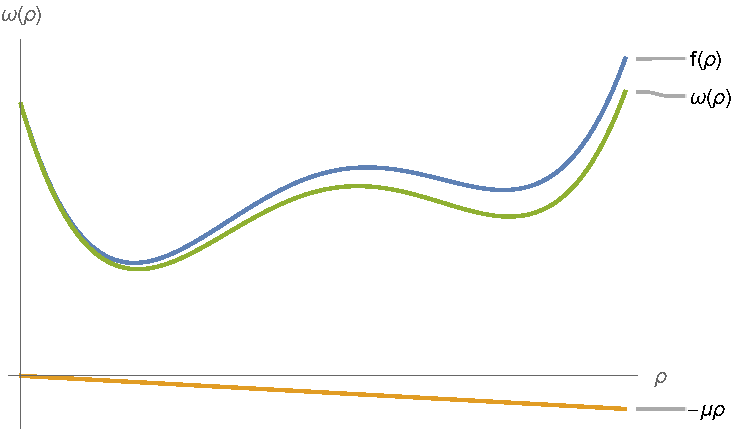
\includegraphics[width=\textwidth]{graphs/vision_with_constraint_1}
         \caption{$\mu < \mu_\text{max}$}
     \end{subfigure}
     \hfill
     \begin{subfigure}[b]{0.3\textwidth}
         \centering
         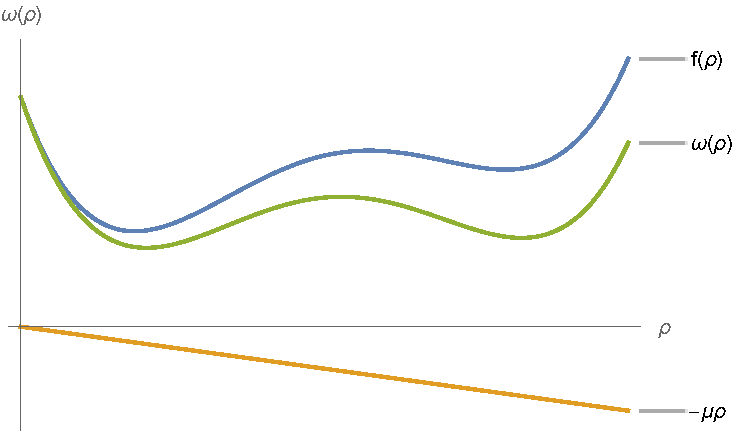
\includegraphics[width=\textwidth]{graphs/vision_with_constraint_2}
         \caption{$\mu = \mu_\text{max}$}
     \end{subfigure}
     \hfill
     \begin{subfigure}[b]{0.3\textwidth}
         \centering
         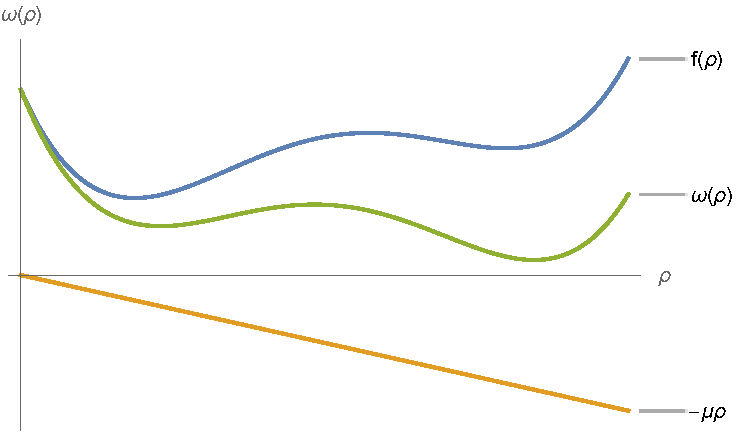
\includegraphics[width=\textwidth]{graphs/vision_with_constraint_3}
         \caption{$\mu > \mu_\text{max}$}
     \end{subfigure}
        \caption{Graphs of the free-energy and pressure for 3 different values of $\mu$.}
\end{figure}

\subsubsection{Example transition of the 2nd order.}
The typical example of 2nd order transition is the polarization/spin without any magnetic field $B$. We know that $m = -\pdv{F}{B}\Big|_{B = 0}$ so we get immediately that:
\[
F(m, B) = F(m) - m B
\]
Again arguing by taking $T$ as a constraint we have:\\
\begin{figure}[h!]
\centering
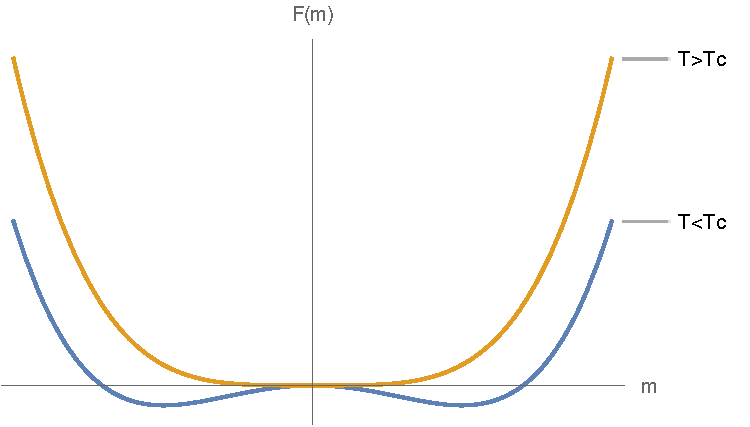
\includegraphics[width = 0.8\textwidth]{graphs/Ex_trans_2nd_order}
\end{figure}
A consequence of this is that:
\[
\chi = \pdv{m}{B}\Bigg|_{B = 0} \stackrel{T\to T_c}{\longrightarrow} \infty
\]
The proof is as follows:
\[
\tilde{F}(m ,B) = F(m) - m B \Rightarrow \pdv{\tilde{F}}{m} = 0 \Leftrightarrow \pdv{F}{m}\Bigg|_{m_\text{eq}(B)} = B
\]
We then rewrite by taking a first order expansion in $m$ and we get:
\[
\pdv{F}{m}\Bigg|\underbrace{(m_\text{eq}(B + \dd B))}_{m_\text{eq}(B) + \dd m_\text{eq}} = B + \dd B \Rightarrow \cancel{\pdv{F}{m}\Bigg|m_\text{eq}(B)} + \pdv[2]{F}{m}\Bigg| x \dd m_\text{eq} = \cancel{B} + \dd B
\]
Which gives:
\[
\chi = \dv{m_\text{eq}}{B} \Bigg|_{B = 0} = \left(\pdv[2]{F}{m}\Bigg|_{B = 0}\right)^{-1} \quad \text{ and when } T \to T_c \text{ we have } \pdv[2]{F}{m}\Bigg|_{B = 0} \to 0 
\]
So we get that $\chi$ diverges at the transition point.
 
\subsection{Transitions of the first order and construction of the double tangent.}
We saw already that for first order transitions we get a discontinuity of the order parameter at the transition point and we also have the following equalities:
\[
\begin{cases}
P_v = P_L\\
\mu_v = \mu_L
\end{cases}
\]
However if we treat the problem as being part of the grand-canonical ensemble we have that $N, V, T$ are fixed, hence $\rho = N/V$ is fixed which seems to contradict the fact that $\rho$ must have a discontinuity at $C$. The way in which this 'paradox' is solved is that the system will become un-homogeneous for $N$ and $V$. Now if you let:
\[
f(\rho, T) = \frac{\mathcal{F}}{V}(N, V, T)
\]
Then stability dictates that:
\[
\pdv[2]{\mathcal{F}}{V} \Bigg|_{T, N} \geq 0 \Rightarrow \pdv[2]{f}{\rho} \Bigg|_T \geq 0
\]
Since:
\[
P = -\pdv{\mathcal{F}}{V} = - \pdv{}{V}\left(V f(\frac{N}{V})\right) = - f + \rho f'(\rho)
\]
Remark also that we could write:
\[
P = - \frac{\Omega}{V} = - \frac{F - \mu N}{V} = -f + \underbrace{\mu}_{\pdv{f}{\rho}} \rho
\]
And furthermore:
\[
\pdv[2]{\mathcal{F}}{V} = - \pdv{P}{V} = - \pdv{}{\rho}\left(-f + \rho f'(\rho)\right) \frac{-N}{V^2} = \frac{N}{V^2}\left[ -f + \rho f'' + f \right]
\]
Then the stability condition can be rewritten as:
\[
0 \leq \pdv[2]{\mathcal{F}}{V} = \frac{1}{V} \rho^2 f''(\rho)
\]
So in conclusion we are requiring that $f$ must be convex for $\rho$. Points for which $f''(\rho, T) = 0$ are called spinodals.

\subsubsection{Double Tangent.}
What we mean by a double tangent is a tangent line that will hit both convex pits of our function $f$, corresponding to the two equilibrium positions. We will now see that the double tangent respects the equilibrium conditions. The tangent in $\rho_0$ must respect the following conditions:
\[
\pdv{f}{\rho}\Bigg|_{\rho = \rho_0} = \mu = \pdv{\mathcal{F}}{N}\Bigg|_{T,V}, \quad y = f'(\rho_0)(x - \rho_0) + f(\rho_0), \quad y(x = 0) = -P(\rho_0)
\]
So the slope of the tangent gives $\mu(\rho_L) = \mu(\rho_v)$ and the coordinate at origin gives that $P(\rho_L) = P(\rho_v)$. What happens physically behind this double tangent is the following. As we said before to circumnavigate the fact that we are fixing $\rho$ the system will split as follows: $\rho = x \rho_v + (1 - x) \rho_L$ which will also give that $f_\text{mix}(\rho) = x f(\rho_v) + (1 - x) f(\rho_L) \leq f_\text{hom}(\rho)$. In other words the system will try to 'convexify' the function by reducing the hill to the double tangent in between two pits. Which gives the following phase diagram:
\begin{figure}[h!]
     \centering
     \begin{subfigure}[b]{0.47\textwidth}
         \centering
         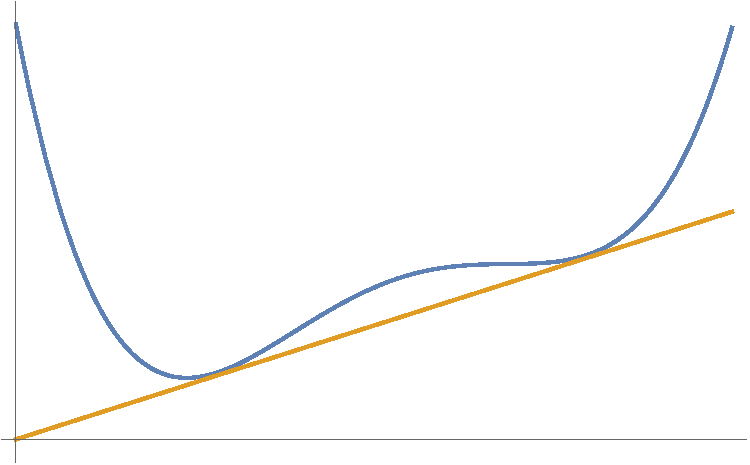
\includegraphics[width=\textwidth]{graphs/double_tangente}
         \caption{Graph of the free-energy with the double tangente.\\ \quad \\ \quad}
     \end{subfigure}
     \hfill
     \begin{subfigure}[b]{0.47\textwidth}
         \centering
         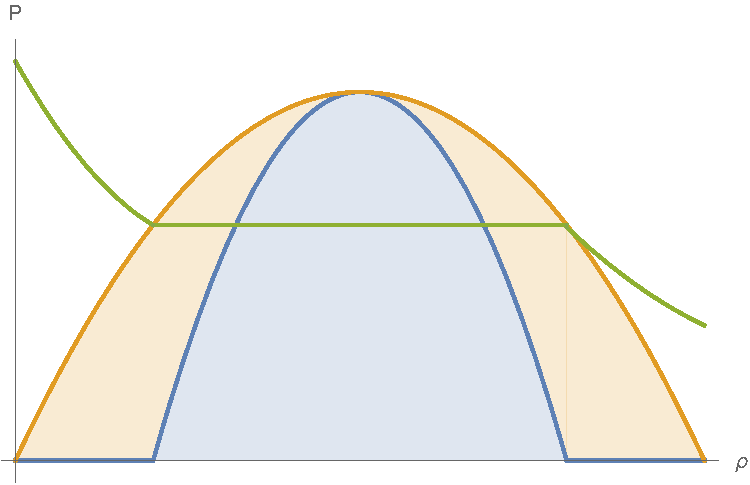
\includegraphics[width=\textwidth]{graphs/double_tangente_phase_diagram}
         \caption{Graph of the phase diagram, the orange zone corresponds to the meta-stable area, the blue zone is the spinodal area. The green line is an isothermic transition.}
     \end{subfigure}
        \caption{Graphs of a 2 minima system.}
\end{figure}
\subsection{Transitions of the second order, critical exponents.}
In the transitions of the second order we can pass continuously from one phase to the other. However at the transition point the length scale of the system will diverge to infinity, and as a consequence physical quantities will behave exponentially:
\[
C_V \sim |T - T_C|^{-\alpha}, \Phi \sim |T - T_C|^\beta, \chi = - \pdv{\Phi}{B} \Bigg|_{B = 0} \sim |T - T_C|^{-\gamma}
\]
What is remarkable is that these exponents $(\alpha, \beta, \gamma, \cdots)$ are universal and depend only on the symmetries of the problem.

\chapter{Systems in interaction and change of phase.}
\section{Introduction.}
\begin{wrapfigure}{R}{0.3\textwidth}
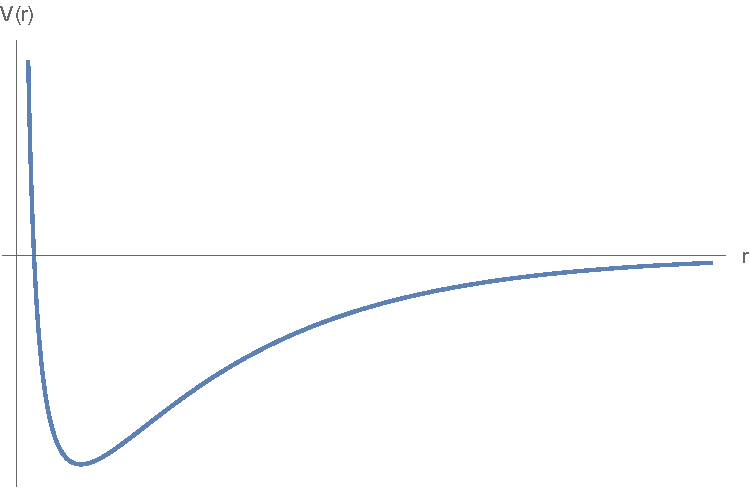
\includegraphics[width = 0.3 \textwidth]{graphs/ExamplePotential}
\end{wrapfigure}
Up to now we have considered only perfect systems that had no interactions. This approximation is more or less valid so long as $\rho \to 0$. More generally two interacting molecules would influence each other with a potential that has probably a shape like the following. A common example is the Lennard-Jones potential:
\[
V(r) = 4 E \left[ \left(\frac{\sigma}{r}\right)^R - \left(\frac{\sigma}{r}\right)^6 \right]
\]
Another simpler example is the hard spheres example:
\[
V(r) = \begin{cases} +\infty \text{ if } r = R\\0 \text{ if } r > R
\end{cases}
\]
Which can also be re-written as:
\[
e^{-\beta V(r)} = H(r - \sigma)
\]
Then the Hamiltonian will be written (assuming the particles interact only by pairs):
\[
\mathcal{H} = \sum_i = \frac{\vec{p}_i^2}{2m} + \sum_{i < j} V(|\vec{r}_i - \vec{r}_j|)
\]
And usually the goal will be to compute or approximate the partition function:
\[
Z = \frac{1}{N! h^{3N}}\int \dd \vec{r}_1 \cdots \dd \vec{r}_N \dd\vec{p}_1 \cdots \dd \vec{p}_N e^{-\beta\mathcal{H}}
\]
A particular system for which we will solve this problem is the one of spins in interaction where the Hamiltonian is given by:
\[
\mathcal{H} = - \frac{4 J_{ij}}{h^2} \vec{s}_i \cdot \vec{s}_j
\]
Heisenberg's model says something similar:
\[
\mathcal{H} = - \frac{4 J_{ij}}{h^2} \vec{s}_i \cdot \vec{s}_j - \gamma \vec{B} \cdot \sum_i \vec{s}_i
\]
Finally Ising's model simply restricts the value of the spin to being only $\pm\frac{\hbar}{2}$ and restricts interactions to only nearest neighbors. Then we have:
\[
\mathcal{H} = - J \sum_{i < j, |i - j| \leq 1} S_i S_j - \mu B \sum_i S_i 
\]

\section{Interactions and partition functions.}
\section{Magnetic systems.}
\subsection{Exact Results in 1D and 2D.}
For the general culture of the reader we include here known exact results in 1D and 2D. 
\subsubsection{1D.}
In 1 dimension if we introduce $\bar{S} = \langle \frac{1}{N} \sum_{i = 1}^N S_i \rangle$ will behave as follows, i.e. there is no phase transition. And the exact result is given by:
\[
\bar{S}  = \frac{\sinh(\frac{\mu B}{k_B T})}{\sqrt{\sinh^2(\frac{\mu B}{k_B T}) + \exp(-\frac{4J}{k_B T})}}
\]

\subsubsection{2D.}
Onsager in 1944 computed the partition function in 2 dimensions and Yang computed the mean polarization 8 years later. The results are as follows:
\[
Z = \left(2 \cosh \frac{2 J}{k_B T} e^I \right)^N,\quad I = \frac{1}{2\pi} \int_0^\pi \dd \phi \log \frac{1 + \sqrt{1 - x^2 \sin^2 \theta}}{2}, \quad x = \frac{2 \sinh (\frac{2J}{k_B T})}{\cosh^2(\frac{2J}{k_B T})}
\]
So there is a phase transition (when $B = 0$) which is the $T_C$ such that:
\[
\sinh \frac{2J}{k_B T_C} = 1
\]
And close to the transition we have that:
\[
\bar{S}(T) = \left(1 - \frac{1}{\sinh^4(\frac{2J}{k_B T})}\right)^{1/8} \Rightarrow S(T \sim T_C) \sim |T - T_C|^{1/8}
\]

\subsection{Ising model in one and two dimensions: exact results.}
\subsection{Mean field approximation.}
The idea of the mean field approximation is to say that "fluctuations are low". So a given value $X$ will not stray far off from $\bar{X}$. We will now show through some examples why this can be useful. First we consider a system without any interactions $J = 0$ but with $B \neq 0$. Then we have:
\[
\mathcal{H} = -\mu B \sum_i S_i, \quad Z = \sum_{\{S_i\}} e^{\mu B \beta \sum_i S_i} = \sum_{S_1 = \pm 1} e^{\mu B \beta S_1} \times \sum_{S_2 = \pm 1} e^{\mu B \beta S_2} \times \cdots = \left(2 \cosh \frac{\mu B}{k_B T}\right)^N
\]
And the mean polarization is given by:
\[
\bar{S} = \frac{\sum_{\{S_i\}} \frac{1}{N} \sum_i S_i e^{\mu B \beta \sum_i S_i}}{\sum_{\{S_i\}} e^{\mu B \beta \sum_i S_i}} =  \frac{1}{N} \pdv{}{x} \log Z = \pdv{}{x} \log(2 \cosh x) = \tanh(\frac{\mu B}{k_B T}) \quad \text{ with } \quad x = \mu \beta B
\]
Now we want to add the interactions. So we get:
\[
\mathcal{H} = - J \sum_{|i - j| = 1} S_i S_j
\]
A way to apply the approximation is to write $S_i = \bar S + \delta S_i$ then the Hamiltonian becomes:
\[
\mathcal{H} = - \frac{J}{2} \sum_{i,j} (\bar{S} + \delta S_i)(\bar{S} + \delta S_j) - \mu B \sum_i S_i = -\frac{J}{2}N^2 \bar{S} - \frac{J}{2}\sum_{i,j}(\bar{S} + \delta S_i + \bar{S} \delta S_j) - \cancelto{\text{negligeable}}{\frac{J}{2}\sum_{i,j} \delta S_i \delta S_j} - \mu B \sum_i S_i
\]
We the mean field approximation is equivalent to saying that we allowed to cancel that 3rd term. Further developing we get that:
\[
\mathcal{H} = \frac{J}{2} q N \bar{S}^2 - (q J \bar{S} + \mu B)\sum_i S_i
\]
So we get that:
\[
\mu_{B_\text{eff}} = \mu B + q J \bar{S}
\]
Then finally we obtain for the mean polarization:
\[
\bar{S} = \tanh\left[\frac{\mu B_\text{eff}(\bar{S})}{k_B T}\right]= \tanh\left[\frac{\mu B + q J \bar{S}}{k_B T}\right]
\]
Which can be re-written as:
\[
\frac{k_B T}{q J} x = \tanh x
\]
Now this equation can be numerically solved and we obtain the figure plotted below.
So that when $\alpha > 1$ we have that the only possible solution is $\bar{S} = 0$. When $\alpha < 1$ then we have 3 possible solutions, and the solution in 0 is unstable. Now for $T \sim T_C$ we know that we can approximate $\tanh$ with:
\[
\tanh x \approx x - \frac{x^3}{3} \Rightarrow \alpha x = x - \frac{x^3}{3} \Leftrightarrow x^2 = 3(1 - \alpha) \Rightarrow S(T) \propto |T - T_C|^{1/2}
\]
Then if we compute the susceptibility we get:
\[
\chi = \dv{\bar{S}}{B}\Bigg|_{B = 0} \sim \frac{1}{|T_c - T|} \stackrel{T = T_c}{\longrightarrow} \infty
\]
\begin{figure}[h!]
\centering
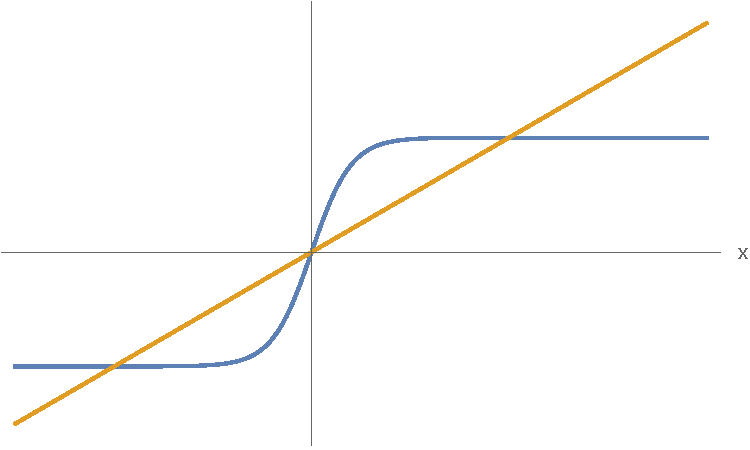
\includegraphics[width = 0.6\textwidth]{graphs/TanhLin_Cut}
\end{figure}

\subsection{Alternative method.}
Another way to get to this result is to pass through the free-energy. We know that for independent spins we have:
\[
H = -\mu B S, \quad Z = \left(2 \cosh \frac{\mu B}{k_B T}\right)^N, \quad F = -k_B T N \log(2\cosh\frac{\mu B}{k_B T})
\]
Now when we take into account the interactions we need to compute:
\[
H = H_{MF} = \underbrace{\frac{J q N \bar{S}^2}{2}}_{\text{cst}} - \mu B_\text{eff} \sum_i S_i, \quad Z_{MF} = \sum_{\{S_i\}} e^{-\beta H_{MF}(S_i)} = e^{-\frac{Jq N \bar{S}^2}{2 k_B T}} \left(2 \cosh \frac{\mu B_\text{eff}}{k_B T}\right)^N 
\]
This then gives:
\[
F_{MF}  = -k_B T\log Z = ...
\]
Note that this can simply be viewed as a free-energy that considers $\bar{S}$ as a constraint. Then we have $F_{MF}(\bar{S})$. Hence to get the equilibrium we have to try and minimize $F$ for $\bar{S}$ which gives:
\[
\pdv{F_{MF}}{\bar{S}} = 0 = N\left(J q \bar{S} - k_B T \frac{J q}{k_B T} \tanh(\frac{J q \bar{S}}{k_B T}) \Rightarrow \bar{S} = \tanh (\frac{J q \bar{S}}{k_B T})\right)
\]
Note that if we plot the free energy as a function we will see that for $T > T_C$ we have something that looks like a polynomial and when $T < T_C$ two minima will appear. What happens is that when $T$ varies the 'courbure' smoothely changes with it as well. Remark that this is a characteristic of transitions of the second order. At the first order instead there is a discontinuity of the minima at the transition.

\subsection{Description of Landau}
Landau tried to generalize the description of any phase change, we will summarize here briefly some of the results. First when we are close to the transition the assumption is that we get:
\[
F_{MF}(\bar{S}) \stackrel{T \sim T_C}{\approx} \frac{1}{2} \alpha(T) (T - T_C) \bar{S}^2 + \frac{1}{4} \beta(T) \bar{S}^4 + \cdots
\]
This is Landau's expansion, i.e the power expansion of the free-energy in the order parameter. This is for second order transitions but we have something similar for first order transitions:
\[
F_{MF}(\phi) = \frac{1}{2} \alpha(T) \phi^2 + \frac{1}{3} \beta(T) (T - T^*) \phi^3 + \frac{1}{4} \gamma(T) \phi^4 + \cdots 
\]
What fixes the powers in the expansion are the microscopical symmetries. Take for example the spin system we studied previously. Note that there is an up/down symmetry, i.e if we switch all the spins the system would be characterized in the same way. In contrast, for example, with the transition from liquid to gas where it is clear that switching from $\rho_L$ to $\rho_G$ clearly does not give the same system. The applications of this are numerous but a few examples are supra-conductivity, liquid crystals, super fluidity. In fact De Gennes first noticed that what Landau derived for supra-conductors could be adapted and applied to liquid crystals. For more details on this we refer to Chaikin-Lubensky.

\subsection{Alternative approach.}
We now present an alternative approach to the mean field approximation, called Bragg-William. We will see that this will not give the same free-energy for example, but one has to remember that the mean field is only an approximation. Hence according to when, or on what, we make an approximation we might get slightly different results but in the end they should turn out to be equivalent. The idea of Bragg-William is to try and quantify the entropy of the system. So we know:
\[
E = \langle H \rangle = - J \langle \sum_{i, j} S_i S_j \rangle = - J \frac{1}{2} \langle \sum_{|i - j| = 1} S_i S_j \rangle \approx - J \frac{N q}{2} \bar{S}^2
\]
Then the entropy should be given as:
\[
\mathcal{S}(\bar{S}) = k_B \log \Omega = k_B \log(\#\{\text{configurations } x | \bar{S}(x) = \bar{S}\})
\]
So the problem is reduced to counting how many ways there are to generate $\bar{S}$. Now if we write:
\[
\bar{S} = \frac{N_+ - N_-}{N}, \quad \text{ where } \quad N_+ = N\left(\frac{1 + \bar{S}}{2}\right), \quad N_- = N\left(\frac{•}{•}\right)
\]
Now the number of possible configurations is simply given by:
\[
\Omega = \begin{pmatrix}
N\\N_+
\end{pmatrix}
= \frac{N!}{N_+!N_-!}
\]
From this we get:
\[
\mathcal{S} = k_B \log \frac{N!}{N_+!N_-!} = k_B \left( N\log N - N - N_+\log N_+ + N_+ - N_-\log N_- + N_-  \right) = -k_B N (\frac{N_+}{N} \log \frac{N_+}{N} + \frac{N_-}{N} \log \frac{N_-}{N}) = -k_B N \left(\frac{1 + \bar{S}}{2}\log \frac{1 + \bar{S}}{2} + \frac{1 -\bar{S}}{2}\log\frac{1-\bar{S}}{2}\right)
\]
So in total we get:
\[
F_{BW}(\bar{S}) = -\frac{JqN\bar{S}^2}{2} + Nk_B T\left(\frac{1 + \bar{S}}{2}\log \frac{1 + \bar{S}}{2} + \frac{1 -\bar{S}}{2}\log\frac{1-\bar{S}}{2}\right)
\]
As we said earlier, remark that this expression of the free-energy is not the same as the one we found previously, however the minima will be the same. We will now compute these minima:
\[
- = \pdv{F_{BW}}{\bar{S}} = - J N q \bar{S} + \frac{N k_B T}{2} \log \frac{1 + \bar{S}}{1 - \bar{S}}
\]
Now note that $\frac{1 + \bar{S}}{1 - \bar{S}} = \exp(\frac{2 J q \bar{S}}{k_B T})$ so plugging this back in we get that:
\[
\bar{S} = \frac{\exp(2 \frac{J q \bar{S}}{k_B T}) - 1}{\exp(2\frac{J q \bar{S}}{k_B T}) + 1} = \tanh(\frac{q J \bar{S}}{k_B T})
\]
So indeed, as predicted, we get the same minima and the same transition point altough the expression of the free-energy is slightly different. Note that what Bragg-Williams is actually doing is:
\[
F = \langle H \rangle - T \mathcal{S}_0
\]
Where $\mathcal{S}_0$ is the entropy of a 'reference' system. What this means is that we are doing an 'expansion' on a simpler model: the model without interactions in our case. And we treat the energy as a perturbation on the previous more basic model.

\section{Network models.}
\subsection{Application to a 1D model of capillary condensation.}
A lattice model for a liquid is simply to consider a square lattice where each square either contains a particle ($S_i = 1$)  or does not contain a particle ($S_i = 0$). We also assume that the interactions in between particles are only effective over short lengths, hence we consider only nearest neighbors. We denote the energy of interaction by $-\epsilon_\times$. Then the Hamiltonian is given by:
\[
H = H(\{S_i\}) = -\epsilon_\times \sum_{|i - j| = 1} S_i S_j
\]
We can also put the whole system in an outside potential of energy $-\epsilon_0$ which acts on all the particles in the same way. This gives an extra term to the Hamiltonian:
\[
H_\text{ext} = - \epsilon_0 \sum_i S_i
\]
Finally the total number of particles is given by:
\[
N = \sum_i S_i
\]
Note that this model is a very rich model that can be used in numerous situations. It is obvious that it will present a phase transition since it is so close to the Ising model, but it is also broader and can be applied more generally.

\subsubsection{Illustration.}
\begin{wrapfigure}{r}{0.2\textwidth}
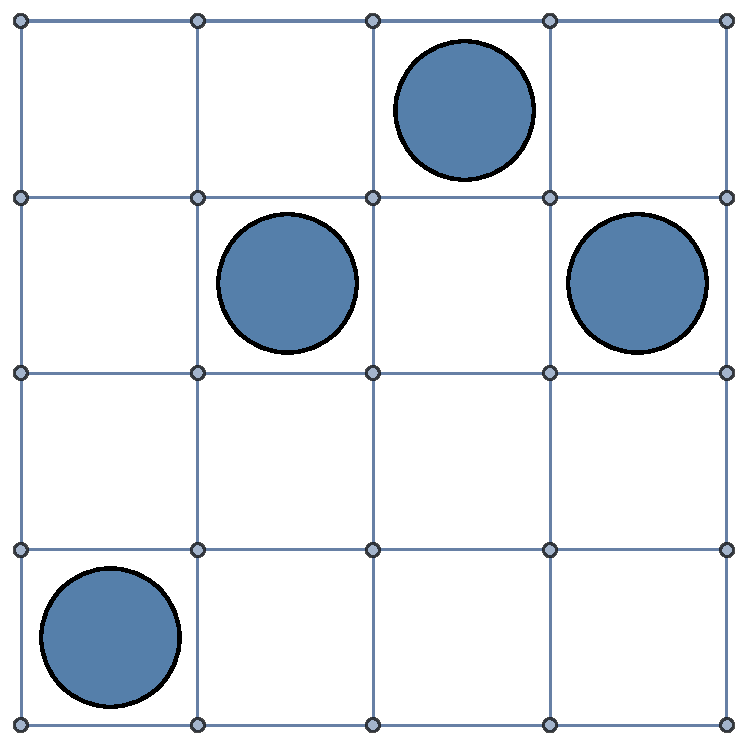
\includegraphics[width = 0.2\textwidth]{graphs/ExampleCappillary}
\end{wrapfigure}
To show an example of the use of this model we will apply it to a 1D capillary condensation model. The idea is that we have two surfaces facing each other at a distance $D$ and a bulk of gas on the side connected to the space in between the surfaces. The surfaces prefer to have a dense liquid in between them while the bulk prefers having a gaseous phase in it. We therefore have a competition in between these two phenomenons and we get the intuition that we will have a phase transition for a certain $D_C$ where for $D > D_C$ the bulk 'wins'  while when $D < D_C$ the surfaces 'win'. What we will use here is a periodic 1D model. We put an interaction term $-\epsilon_0$ in between the surface and the particles, denote $M$ the number of cells of our lattice and $\epsilon_\times$ the energy of interaction, finally by periodic we intend that $S_{M+1} = S_1$. Then the Hamiltonian is given by:
\[
H_{1D} = -\epsilon_\times \sum_{i = 1}^M S_i S_{i +1} - \epsilon_0\sum_{i = 1}^M S_i
\]
Remark that if we try to fix the number of particles: $N = \sum_i S_i$ the computations for the Hamiltonian will be atrocious since we already have a dependence on the sum of the $S_i$. That is why we choose to work in the grand-canonical so as to not fix the number of particles. Then:
\[
\Theta = \sum_N e^{\frac{\mu N}{k_B T}} Z_N = \sum_{S_1 = 0, 1} \sum_{S_2 = 0, 2} \cdots e^{\frac{\mu}{k_B T} \sum_i S_i} e^{- \frac{H(\{S_i\})}{k_B T}} = \sum_{S_1 = 0, 1}\cdots \sum_{S_M = 0,1} \exp(\frac{\epsilon_\times}{k_B T} \sum_{i = 1}^M S_i S_{i + 1} + \frac{\epsilon_0 + \mu}{k_B T}\sum_{i = 1}^M S_i)
\]

\subsubsection{Computation of $\Theta$ by the transfer matrix method.}
The trick to solve this is to introduce the following:
\[
T(S_i, S_j) = \exp(\frac{\epsilon_\times}{k_B T} S_i S_j + \frac{\epsilon_0 + \mu}{k_B T} \frac{S_i + S_j}{2})
\]
Then note that we can rewrite the partition function as:
\[
\Theta = \sum_{S_1 = 0, 1}\cdots\sum_{S_M = 0, 1} \prod_{i = 1}^M T(S_i,S_{i+1})
\]
Note that from how we defined $T$ we see that it resembles closely to a matrix and in fact:
\[
\sum_{S_k} T(S_i, S_k) T(S_k ,S_j) = (\Pi^2) (S_i, S_j), \quad \text{ where } \Pi = \begin{pmatrix}
T(1, 1) & T(1, 0)\\
T(0, 1) & T(0, 0)
\end{pmatrix}
\]
Then we can rewrite our partition function as:
\[
\Theta = \sum_{S_1 = 0,1} (\Pi^M ) (S_1, S_1) = \Tr (\Pi^M)
\]
Now to compute the trace of this matrix we simply diagonalize it. The matrix itself is:
\[
\Pi = \begin{pmatrix}
\exp(\frac{\epsilon_\times}{k_B T} + \frac{\epsilon_0 + \mu}{k_B T}) & \exp(\frac{\epsilon_0 + \mu}{2 k_B T})\\
\exp(\frac{\epsilon_0 + \mu}{2 k_B T}) & 1
\end{pmatrix}
\]
Note that it is symmetric so it will for sure be diagonilizable now computing the eigen-vectors [...] we get:
\[
\lambda_{\pm} = \frac{1 + a \pm \sqrt{(1 - a)^2 + 4b^2}}{2}
\]
Then we simply get that:
\[
\Theta = \lambda_+^M + \lambda_-^M \stackrel{M \to \infty}{\approx} \lambda_+^M
\]
Then:
\[
\Omega(\mu, T, M) = - k_B T \log \Theta = - M k_B T \log(\lambda_+(\mu, T))
\]
Then in order to compute the average density we do:
\[
N = - \pdv{\Omega}{\mu} = M k_B T \frac{\pdv{}{\mu} {\lambda_+ (\mu, T)}}{\lambda_+(\mu, T)} \Rightarrow \rho = \frac{N}{L} = \frac{k_B T}{a} \frac{\pdv{\lambda_+}{\mu}}{\lambda_+}
\]
Plugging all the results in this gives:
\[
\rho(\mu, T) = \frac{1}{2 a} \left[ 1 + \frac{\sinh(\frac{\epsilon_0 + \epsilon_\times + \mu}{2 k_B T})}{\sqrt{\exp({-\frac{\epsilon_\times}{k_B T}}) + \sinh^2(\frac{\epsilon_0 + \epsilon_\times + \mu}{2 k_B T})}} \right]
\]

\begin{figure}[h!]
\centering
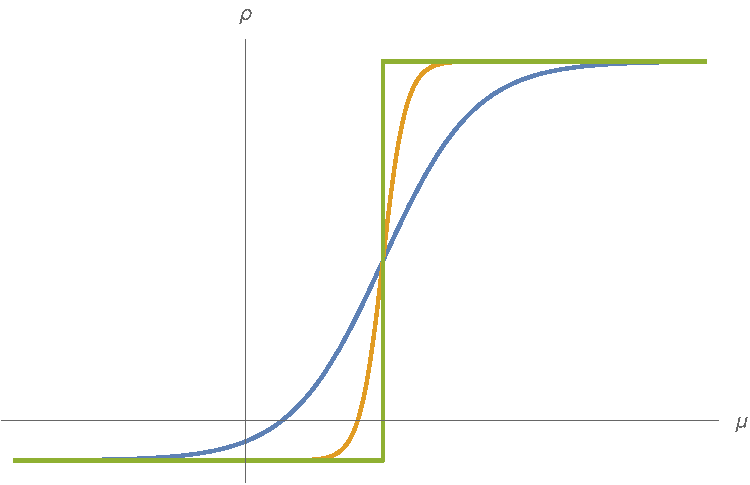
\includegraphics[width=0.6\textwidth]{graphs/CappillaryTransition}
\end{figure}
This might seem as something that is not that impressive but one has to appreciate that this is an exact result. Which means that it is an exact analytical solution to a problem that has a non-trivial interaction phenomenon. Now if we plot $\rho$ we get the figure plotted below. We see that we don't have any discontinuities, hence we do not have any real phase transition. However it is clear that we pass from a low density (gaseous system) to a high density (liquid system). Furthermore the transition becomes steeper and steeper as $\epsilon_\times \gg \epsilon_0$ and for $\epsilon_\times \to \infty$ we will get a step-function. \vspace{10cm}

\section{Dense Liquids and Phase Transitions.}
\subsection{Structures in liquids.}
We define a liquid as being an un-ordered, dense and dynamic phase. To give some orders of magnitude, notice that $\rho \sim \frac{1}{\sigma^3}$ where $\sigma$ is the size of one molecule. So for water par example: $\rho = 3 \cdot 10^{28} \text{molecules}.\text{m}^{-3}$ and $\frac{1}{\sigma^3} = \frac{1}{(3 \cdot 10^{-10})^3} = 3 \cdot 10^{28} \text{molecules}.\text{m}^{-3}$. This is what makes all the complexity of the problem. We saw previously how complicated computing anything with an interaction was, here the behavior of the whole system is determined by these numerous interactions that have much more complex writings. A typical interaction potential would be similar to the one we saw previously in section 8.1. And this is still even considering that particles interact only in pairs.  The easiest case is when we take the extremely hard approximation that particles are simply hard spheres. Then the potential is simply given by:
\[
V(x) = \begin{cases}
+ \infty \quad &\text{ if } x \leq \sigma\\
0 \quad &\text{ if } x > \sigma
\end{cases}
\]
Nonetheless, even such an approximate model presents very interesting behaviors. For example the hard spheres present a liquid-crystal transition, which was one of the first discoveries made using numerical simulation.

\subsubsection{Even correlation function.}
For the following we are now going to introduce a tool that is very widely used in liquid studies. It is denoted $g(r)$, and it denotes the ratio of density of particles at a distance $r$ from a particle. Hence $\rho \cdot g(r)$ gives the density of particles at a distance $r$ from a particle situated at $r = 0$. Another way of writing this is:
\[
\rho^{(1)}(\vec{r}) = \langle \sum_{i = 1}^N \delta(\vec{r} - \vec{r}_i ) \rangle \quad \text{ with } \quad \int \dd^3 \vec{r} \rho^{(1)}(\vec{r}) = \langle \sum_{i = 1}^N \int \dd^3 \vec{r} \delta(\vec{r} - \vec{r}_i) \rangle = N
\]
This is the single body density, it is also possible to define a two-body density as follows:
\[
\rho^{(2)}(\vec{r}, \vec{r}') = \langle \sum_{i \neq j} \delta(\vec{r} - \vec{r}_i) \delta (\vec{r} - \vec{r}_i) \rangle \quad \text{ and when } \quad |\vec{r} - \vec{r}'| \to +\infty, \text{ then } \rho^{(2)}(\vec{r}, \vec{r}') \to \rho^2
\]
Then the even correlation function is given by:
\[
\rho^{(2)}(\vec{r}, \vec{r}') = \rho^2 g(|\vec{r} - \vec{r}'|)
\]
In a dense liquid we expect the following for $g(r)$: [INSERT GRAPH]. For more detail on this we invite the reader to go check Hansen - Mc Donald "Liquid Theory". At a lower density we expect the particles to simply follow a Boltzmann distribution, which gives that $g(r) = e^{-\frac{V(r)}{k_B T}}$  hence something of the sort: [INSERT GRAPH].

\subsubsection{Link with thermodynamics.}
It turns out that in numerous problems the correlation function is 'the' value to compute since many properties can be derived from it. For example the Viriel formula for pressure is given by:
\[
\frac{P}{k_B T} = \rho - \frac{\rho^2}{6 k_B T} \int \dd \vec{r} \,\,\vec{r} \cdot \vec{\grad} v \,g(r)
\]

\subsubsection{Viriel Expansion}
The previous exact formula can be used as a basis for an expansion in $\rho$. If we assume that $g(r)$ is independent of $\rho$ then we simply get terms in $\rho$ and $\rho^2$. If we consider the first correction of $g$ then we also get a term in $\rho^3$, etc. Hence we can write:
\[
\frac{P}{k_B T} = \rho + B_2 \rho^2 + B_3 \rho^3 + \cdots \text{ where } B_i \text{ is called the Viriel coefficient.}
\]
Then $B_2$ for example takes into account only 2 body interactions and can be computed to be:
\[
B_2 = \frac{1}{2}\left( \int \dd^3 \vec{r} \left[1 - e^{-\frac{V(r)}{k_B T}}\right] \right)
\]
There are two possible proofs for this. The first is to directly take the Viriel formula and we inject the first correction in $g$ independent of the density. Then $g(r) = g_0(r) = \exp(-\frac{V(r)}{k_B T})$, we then get the desired result:
\[
-\frac{1}{6 k_B T} \int \dd \vec{r}\,\, \vec{r} \cdot \underbrace{\vec{\grad} v e^{-\frac{V(r)}{k_B T}}}_{k_B T \left(1 - e^{-\frac{V(r)}{k_B T}}\right)} = \frac{-1}{6 k_B T} \int \dd \vec{r} \,\, \vec{r} \cdot \vec{\grad} \left[ 1 - e^{-\frac{V(r)}{k_B T}} \right] = \underbrace{\int_{R \to +\infty} \dd \vec{S} \, \vec{r} (1 - e^{-\frac{V(r)}{k_B T}})}_{\to 0} + \frac{1}{6} \int \dd^3 \vec{r} (1 - e^{-\frac{V(r)}{k_B T}}) \underbrace{\vec{\grad} \cdot \vec{r}}_{3}
\]
Which gives:
\[
B_2 = \frac{1}{2} \int \dd^3 \vec{r} (1 - e^{-\frac{V(r)}{k_B T}}
\]
The second way to compute this is to develop the partition function (Mayer development). We will do here only a 'cheap' version of the Mayer development. We write $Z = z_\text{id} \times Z_\text{ex}$ where:
\[
Z_\text{id} = \frac{1}{N!}\left(\frac{V}{\lambda^3_T}\right)^N \quad \text{ and } \quad Z_\text{ex} = \frac{1}{V^N} \int \dd^3 \vec{r}_1 \cdots \dd^3\vec{r}_N \, e^{-\beta \sum_{i < j} V(\vec{r}_{ij})}
\]
Then we re-write:
\[
Z_\text{ex} = \langle e^{-\sum_{i < j} \beta V(r_{ij})} \rangle_v \quad \text{ where } \quad \langle \cdot \rangle_v = \frac{1}{V^N} \int \dd \vec{r}_1 \cdots \dd \vec{r}_N (\cdot)
\]
We can then simplify this by saying that $e^{-\beta V(r_{ij})} = 1 + f(r_{ij})$ which gives:
\[
Z_\text{ex} = \langle \prod_{i < j} e^{-\beta V(r_{ij})} \rangle_v \approx \prod_{i < j} \langle e^{-\beta V(r_{ij})}
\]
Where in the approximation we simply kept only the two body interaction terms, i.e only the terms that were linear in $f$. Now we notice that:
\[
\langle e^{-\beta V(r_{ij})}\rangle_v = \frac{1}{V^N} \int \dd \vec{r}_1 \cdots \dd \vec{r}_N e^{-\beta V(r_{ij})} = \frac{1}{V^2} \underbrace{\int \dd \vec{r}_1 \dd \vec{r}_2 e^{-\beta V(\vec{r}_{12})}}_{\vec{r}_{12} = \vec{r}_1 - \vec{r}_2 = \vec{r}} = \frac{1}{V} \int \dd \vec{r} \underbrace{e^{-\beta V(\vec{r})}}_{1 + (e^{-\beta V(r)} - 1)} = 1 - \frac{1}{V} \left(\int \dd \vec{r} (1 - e^{-\beta V(\vec{r})}) \right)
\]
Now computing the free-energy we get that:
\[
F = -k_B T \log Z = F_\text{id} - k_B T \log  \underbrace{\prod_{i < j} \left[1 - \frac{1}{V}\left(\int \dd \vec{r} (1 - e^{-\beta V(r)}) \right) \right]}_{\left(1 - \frac{1}{V} \int \dd \vec{r} 1 - e^{-\beta V(r)}\right)^{\frac{N(N-1)}{2}}} = F_\text{id} - \frac{k_B T}{2}N^2 \log \underbrace{\left(1 - \frac{1}{V} \int \dd \vec{r} [1 - e^{-\beta V(r)}]\right)}_{\approx \frac{-1}{V} \left( \int \dd \vec{r} 1 - e^{-\beta V(r)}\right)}
\]
Hence we get that:
\[
P = - \pdv{F}{V} = P_\text{id} + P_\text{ex} = \rho k_B T + k_B T \rho^2 \frac{1}{2} \int \dd \vec{r} (1 - e^{-\frac{V(r)}{k_B T}})
\]

\subsection{Viriel expansion and Van der Waals fluid.}
\subsection{Liquid-Gas transition in Van der Waals fluids.}
The idea here is to split the potential in two pieces, a close range interaction term and a long range interaction term. Then we try to compute $B_2(T)$ and we write it as:
\[
B_2 \approx B_\text{SR} + B_\text{LR} \quad \text{ where } \quad B_\text{SR} = \frac{1}{2} \int_{r = 0}^\sigma (1 - \underbrace{e^{-\beta V(r)}}_{ \approx 0}) \text{ and } B_\text{LR} = \frac{1}{2} \int_{r = \sigma}^{+\infty} \underbrace{(1 - e^{-\beta V(r)}}_{\approx \beta V(r)} 
\]
Hence we get that:
\[
B_2 = \frac{1}{2} \frac{4 \pi \sigma^3}{3} + \frac{1}{2 k_B T} \int_\sigma^{+\infty} V(r) \dd \vec{r} = b - \frac{a}{k_B T}
\]
We call $b$ the excluded volume and $a$ is positive if the long range potential is attractive.

\subsubsection{State equation.}
From the viriel expansion we immediately get:
\[
\frac{P}{k_B T} = \rho + (b - \frac{a}{k_B T}) \rho^2
\]

\subsubsection{Excluded Volume.}
We can write the above equation as:
\[
\frac{P}{k_B T} = (\rho + b \rho^2) - \frac{a\rho^2}{k_B T}
\]
Note that the problem here is that the second term is valid only at long distance and does not take into consideration the fact that there is a restriction on the volume that a particle can occupy.

\subsubsection{Free Volume.}
A simple way to remedy to this is to simply replace the volume we are considering by what we call the free volume i.e:
\[
V^N \rightarrow V_\text{free}^N = [V - \frac{1}{2} N V_0]^N \text{ where } V_0 \text{ is the volume of 1 particle.}
\]
Hence we get that:
\[
Z = ....
\]
Which gives for the free energy:
\[
F = -k_B T \log Z = - k_B T \log Z_\text{id} - k_B T \log Z_\text{ex} \text{ with } Z_\text{id} = \frac{V^N}{N! \lambda^N_T} \text{ and } Z_\text{ex} = \frac{1}{V^N} (V - \frac{1}{2}N V_0)^N
\]
Hence the pressure is given by:
\[
P = -\pdv{F}{V} = \rho k_B T + N k_B T \pdv{}{V} \log(1 - \frac{N V_0}{2 V}) = \rho k_B T + \frac{\rho^2 k_B T}{1 - \frac{\rho V_0}{2}} \frac{V_0}{2} = \frac{\rho k_B T}{1 - b \rho}
\]
Where $b = \frac{V_0}{2}$ is the excluded volume. Note that now as expected the pressure will diverge for a density that goes to $\frac{1}{b}$ since the volume is being saturated, hence the free volume will go to zero.

\subsubsection{Regrouping all the terms.}
Putting everything together we get that:
\[
P = \frac{\rho k_B T}{1 - b \rho} - a \rho^2
\]
Which also gives:
\[
f = \frac{F}{V} = k_B T [\rho \log \frac{\rho \lambda^3_T}{1 - b \rho} - \rho] - a \rho^2
\]
These are what is called the pressure and free energy equation for a Van der Waals gas. 

\subsection{Transition gas-liquid of Van der Waals fluid.}
\subsubsection{Thermodynamic properties.}
We have $P(\rho, T)$ and $\mu = \pdv{f}{\rho}\Bigg|_{V, T}$ which gives:
\[
\mu = k_B T \log (\rho \lambda^3_T)  + \pdv{}{\rho} \left[k_B T \log \frac{1}{1 - b \rho} - a \rho^2\right] = k_B T \log(\frac{\rho \lambda^3_T}{1 - b \rho}) + k_B T\frac{\rho b}{1 - b \rho} - 2 a \rho
\]
But we immediately see here that we are going to have a problem. At high temperature we see immediately that we can neglect $a \rho$ since the rest is going to dominate. And we are going to get a function of this kind: [INSERT GRAPH]. However as seen previously the section where $P$ is decreasing is a highly unstable zone. We denote this zone by $\rho_\text{spin}^V$ and $\rho_\text{spin}^L$. This is what is called the \textbf{spinodal}, it is the limit of thermodynamic stability and the two bounds: $\rho_\text{spin}^{V,L}$ are solution of $\pdv{P}{\rho} = 0$. We can compute these:
\[
0 = \pdv{P}{\rho} = \frac{k_B T}{1 - b \rho} + \frac{\rho k_B T b}{(1 - b \rho)^2} - 2 a\rho \Rightarrow k_B T = 2 a \rho(1 - b \rho)^2
\]
We can then plot the spinodal zone: [INSERT GRAPH], within which all behavior will be unstable. Note that at the top there is a point $(C)$ where the two spinodal limits will be equal to each other, i.e the maximum of the peak and the minimum of the 'cuvette' will overlap. Mathematically this gives the condition $\rho_\text{spin}^V = \rho_\text{spin}^L$, which is also written (using the second definition):
\[
\pdv{P}{\rho} = 0 \quad \text{ and } \quad \pdv[2]{P}{\rho} = 0
\]
Then:
\[
\pdv[2]{P}{\rho} = \frac{2 k_B T}{(1 - b \rho)^2} - 2 a
\]
Which gives the following conditions:
\[
\begin{cases}
k_B T_c = 2 a \rho_c (1-  b \rho_c)^2\\
b k_B T_c = a (1 - b \rho_c)^3
\end{cases}
\Rightarrow \begin{cases}
b = \frac{1}{2 \rho_c} (1 - b \rho_c)\\
\rho_c =\frac{1}{3 b}
\end{cases} \Rightarrow \begin{cases}
\rho_c = \frac{1}{3b}\\
k_B T_c = \frac{8a}{27 b}\\
P_c = \frac{a}{27 b^2}
\end{cases}
\]

\subsubsection{Coexistence.}
If we now plot the volumic free energy we get: [INSERT GRAPH]. Where we see that for $T > T_C$ we will have a convex function, while for $T < T_C$ we will two minima and as we did previously we need to construct the double tangent to the two minima in order to find the critical values. This has no analytical solution and has to be done numerically.

\subsection{Thermodynamic of capillary condensation.}
The definition of this phase transition is the transition from liquid to gas in a confined space. When we try to make the experiment using a "BET" isotherme we get the following results:
\begin{figure}[h!]
\centering
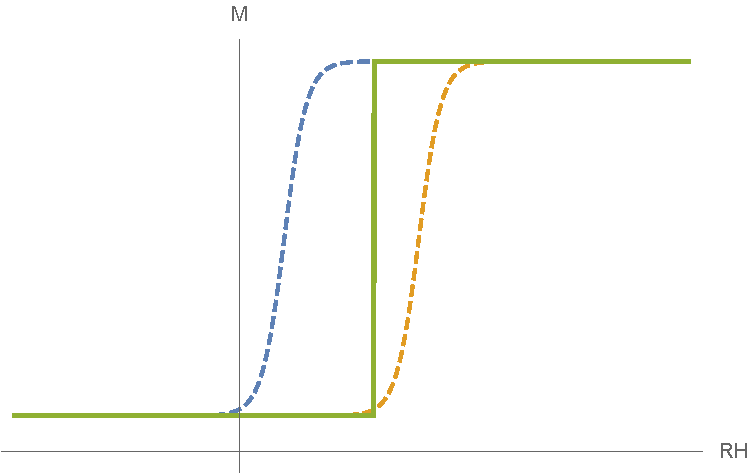
\includegraphics[width = 0.6\textwidth]{graphs/capillaryCondensationBET}
\end{figure}
The physical principle behind this is that the vapor phase is stable and has for free energy $\alpha V \Delta f$. However since the surface is what is called a 'wetting' surface it prefers liquid i.e. $\gamma_{SL} < \gamma_{SV}$. Where $\gamma$ is the free energy per unit surface for the interfaces $S-L$ and $S-V$. Hence the energy gain of passing from $L$ to $V$ is given by: $S (\gamma_{SL} - \gamma_{SV})$ where $S$ is the 'wetting' surface. Hence the transition will appear when the gain outweighs the cost i.e. $V \delta f \sim S \delta \gamma$ hence we can introduce $H_c = \frac{V}{S} \sim \frac{\Delta \gamma}{\Delta f}$ which is the parameter that will allow to model the phase transition.

\subsubsection{More precisely.}
There are 2 possible ways to go for this problem. The first is to use the free energy and the second to use a thermodynamic approach. 
\subsubsection{Free Energy Approach.}
The free energy approach is actully a very simplified version of a much more general theory named DFT: "density functional theory". To model the system we introduce a potential that is dependent only on the distance of a particle from the surface called $V_\text{ext}(z)$ then we have something that looks as follows:
\begin{figure}[h!]
\centering
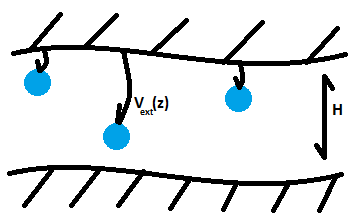
\includegraphics[width = 0.6\textwidth]{graphs/capillaryCondensationDFT}
\end{figure}
Then this gives the following form for the $\Omega$:
\[
\Omega(\rho, \mu, V, T) = \int \dd^3 \vec{r}\left[ f(\rho(\vec{r}) - \mu \rho(\vec{r}) + \rho(\vec{r}) V_\text{ext}(\vec{r}) \right]
\]
Here we make a simplification that says $\rho(\vec{r}) \approx \rho_0 = \text{cst}$. This then simplifies the integral as follows:
\[
\int \dd^3 \vec{r} \rho(\vec{r}) V_\text{ext}(\vec{r}) \approx \rho_0 S \cdot 2 \int_\sigma^{+\infty} \dd z V_\text{ext}(z)
\]
And we define:
\[
-\alpha = \int_\sigma^{+\infty} \dd z V_\text{ext}(z) < 0
\]
Then coming back to the grand potential we get:
\[
\Omega(\rho, \mu, V, T) = V(f(\rho_0) - \mu \rho_0) - 2 \rho_0 S \alpha
\]
Now introducing the parameter that we had an intuition would describe the transition: $H = \frac{V}{S}$ we can rewrite the above equation as:
\[
\Omega = V \left[ f(\rho_0) - \underbrace{\left(\mu + \frac{2\alpha}{H}\right)}_{\mu_\text{app}} \rho_0 \right]
\]
We know that for $\mu < \mu_\text{sat}$ the vapor phase is stable in the reservoir however the apparent chemical potential $\mu_\text{app} = \mu + \frac{2\alpha}{H}$ could be bigger than $\mu_\text{sat}$. Remark also that $f(\rho) = f_\text{VdW}(\rho)$ which we have already treated earlier. Hence we can directly deduce that for $\mu_\text{app} = \mu + \frac{2\alpha}{H} > \mu_\text{sat}$ we will observe a vapor to liquid transition. So if we define $\Delta \mu = \mu_\text{sat} - \mu > 0$ the transition happens for $\Delta \mu = \frac{2 \alpha}{H}$. If we want to re-write this in terms of $\gamma_{SL}$ and $\gamma_{SV}$ we have to first define them. In the considered model we have that $\gamma_{SL} = \rho_L \cdot (-\alpha)$ and $\gamma_{SV} = \rho_V \cdot (-\alpha)$. Hence combining the two writings we can find an expression for alpha:
\[
\alpha = \frac{\gamma_{SV} - \gamma_{SL}}{\rho_L - \rho_V} > 0
\]
Then the transition will appear for:
\[
\Delta \mu = \frac{2 \Delta \gamma}{\Delta \rho H}
\]
Finally we want to define what exactly is 'humidity'. The relative humidity denoted RH is given by:
\[
\text{RH} = \frac{P_v}{P_\text{sat}}
\]
So for example the expression for a perfect gas we have:
\[
\mu = \mu_0  + k_B T \log \frac{P_v}{P_0} \quad \land \quad \mu = \mu_\text{sat} + k_B T \log \frac{P_v}{P_\text{sat}}
\]
Hence we can re-write:
\[
\Delta\mu = k_B T \log (\text{RH}^{-1})
\]
Now note that we can observe different parameters provoking a phase transition. If we fix $H$ then varying RH we can have a phase transition. We can also fix RH and vary $H$ and observe a phase transition. For example if we consider two very rough grains in contact, since the distance in between the extremities will vary according to where we are situated then we will observe some zones where there will be condensation and others where there is not.

\subsubsection{Thermodynamical approach.}
We now want to restudy the same problem but using a thermodynamical approach. The first question one has to ask himself is what is interesting thermodynamic potential to consider to characterize the phase transition? We are working at fixed $V$ and $T$ and what is varying is $\mu$ hence we introduce a function $\Omega(\mu, V, T)$ then we write $\Omega_V$ the potential of the vapor phase and $\Omega_L$ the potential of the liquid phase. Then we have the following relations:
\[
\Omega_V = - P_v V + 2 \gamma_{SV} S \quad \land \quad \Omega_L = - P_L V + 2 \gamma_{SL} S
\]
And $P_V$ and $P_L$ both depend on $\mu$ and $T$. Then the potential difference is given by:
\[
\Delta \Omega = -(P_L - P_V) V - 2(\gamma_{SV}- \gamma_{SL}) S \Leftrightarrow \frac{\Delta \Omega}{S} = -(P_L - P_V) H - 2 \Delta \gamma
\]
So for $\mu, T$ fixed we get:
\begin{figure}[h!]
\centering
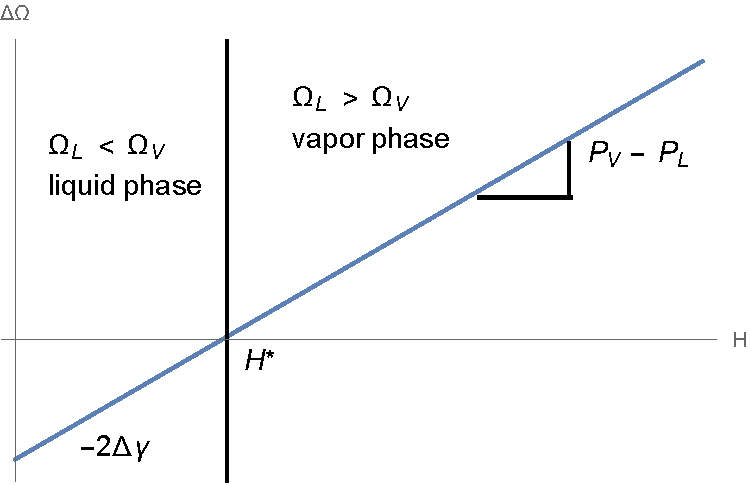
\includegraphics[width = 0.6\textwidth]{graphs/CC_thermo}
\end{figure}
Hence we get a transition for $\frac{H^*}{\Delta \Omega} = 0$ which gives: $H^* = \frac{2 \Delta \gamma}{P_V - P_L}$. The question now is to try and determine $(P_V - P_L)$ as a function of $\mu, T$. We know that:
\[
\mu = \mu_\text{sat} + k_B T \log \frac{P_V}{P_\text{sat}} \Rightarrow P_V = P_\text{sat} \exp(-\frac{\Delta \mu}{k_B T}) \approx P_\text{sat} - \rho_V \Delta \mu \quad \text{ with } \rho_V = \frac{P_\text{sat}}{k_B T}
\]
Now for $P_L$ we cannot use the perfect gas approximation because the pressure and density are way too high. However we can use the Gibbs-Duhem relation, which gives:
\[
\rho \dd \mu = \dd P 
\]
If we furthermore add the hypothesis that liquid is incompressible then we have that $\rho = \rho_L$ which is independent of $\mu$ hence we can rewrite the above equation as:
\[
\rho_L \underbrace{(\mu - \mu_\text{sat})}_{-\Delta \mu} \approx P_L - P_\text{sat}
\]
So overall we get that:
\[
P_V -P_L = P_V - P_\text{sat} + P_\text{sat} - P_L = -\rho_V \Delta \mu + \rho_L \Delta \mu = (\rho_L - \rho_V) \Delta \mu
\]
In conclusion putting everything together we get that:
\[
H^* = \frac{2 \Delta \gamma}{(P_V - P_L)} = \frac{2 \Delta \gamma}{\Delta \rho \Delta \mu}
\]

\subsubsection{Applications.}
An example of this is the (de)pressure in a condensed film. Putting in the numerical values we get that $P_L \sim 10^5 \text{atm}$ which gives an idea of how large $P_L$ can be. Note also that the reverse process also exists i.e. a capillary evaporation. The situation is the same but with hydrophobic surfaces and we reverse all the inequalities we had before. This system is actually something that is extremely important in biology in the study of proteins, because it explains the hydrophobic attraction that is very widely used in biological systems.
\section{Charged systems.}
\subsection{'Ecrantage', free energy.}
\subsection{Ionic phase transition.}

\chapter{Quantum statistics.}
In a way quantum statistics is almost easier than classical statistics because contrary to the classical case everything is always discrete. Hence for example the $N!$ (Gibbs Paradox) or the discretization of the phase space are problems that do not appear anymore. Furthermore in quantum statistics we will always use the grand canonical ensemble, for the simple reason that it is the only ensemble where calculus is doable in a realistic way.

\section{Quantum states and partition functions.}
We could summarize quantum physics by saying that we are passing from the concept of 'particles' to the concept of 'waves'. We have already introduced the De Broglie wavelength:
\[
\lambda_T = \sqrt{\frac{h^2}{2 \pi m k_B T}}
\]
We are in a 'classical' case when $\lambda_T < \text{ distance in between particles } \sim \rho^{-1/3}$. However when $\lambda_T \sim \rho^{-1/3}$ i.e. we are at 'low temperatures' quantum effects appear. We denote by $\ket{\psi}_i$ the wavefunction associated to the state $i$ and we have $\hat{H}\ket{\psi}_i = E_i \ket{\psi}_i$.  The difficulty of the quantum aspects comes from the fact that we have a 'double statistics'. We first have a statistic due to the quantum effects and their uncertainty to which we add the statistics of the problem itself. So for example for a variable $A$ it's average will be given by:
\[
\bar{A} = \sum_{i \text{ quantum states}} p_i \bra{\psi_i} A \ket{\psi_i}
\]
We introduce what is called a density operator which will be very useful in the future:
\[
\rho = \sum_{i \text{ quantum states}} p_i \op{\psi_i}
\]
Then using this operator we can write:
\[
\bar{A} = \Tr (\rho A)
\]
The proof of this is quite simple:
\[
\Tr(\rho A) = \sum_k \bra{k} \rho A \ket{k} = \sum_{k, i} p_i \bra{k}\ket{\psi_i} \bra{\psi_i} A \ket{k} = \sum_i p_i \bra{\psi_i} A \underbrace{\left(\sum_k \op{k}\right)}_{\text{Id}} \ket{\psi_i} = \sum_i p_i \bra{\psi_i} A \ket{\psi_i} = \bar{A}
\]
Note also that:
\[
p_i = \bra{\psi_i} \rho \ket{\psi_i} \quad \land \quad \bra{\psi_i} \rho \ket{\psi_j} = 0 \text{ if } i \neq j
\]
We now start to introduce the statistical physics.
\subsection{Ensembles}
\subsubsection{Micro-canonical.}
We have immediately that the probability of a given state is given by: $p_i = \frac{1}{\Omega}$ where:
\[
\Omega = \sum_{\text{quantum states}} 1
\]
\subsubsection{Canonical.}
We get immediately that:
\[
p_i = \frac{1}{Z} e^{-\beta E_i} \quad \text{ where } \quad Z = \sum_{i \text{ quantum states}} e^{-\beta E_i} = \Tr[e^{-\beta H}]
\]
\subsubsection{Grand Canonical.}
We get similarly that:
\[
p_i = \frac{1}{\Theta} e^{\frac{-E_i + \mu n_i}{k_B T}} \quad \text{ where } n_i \text{ is the degeneracy of the state } i
\]
And we have:
\[
\Theta = \sum_{i \text{ quantum states}} e^{-\beta E_i + \beta \mu n_i} = \Tr[e^{-\beta(H - \mu N)}]
\]

\section{Two examples:}
\subsection{Harmonic Oscillator.}
We take $N$ sites on a lattice and to each site we associate a harmonic oscillator. All the oscillators are independent and have for characteristic frequency $\omega_0$. Then there are $6N$ degrees of freedom in total and the classical system would predict that we have $E = 3Nk_B T$ and $C = 3Nk_B$ however we will see that this will not hold anymore at low temperatures. In the quantum consideration we have that the energies of a harmonic oscillator are given by: $E_n = \hbar \omega_0 (\frac{1}{2} + n)$. Then the partition function will be given by:
\[
Z = \sum_{\text{states } i} e^{-\beta E_i} = \left(\sum_{\text{1D states } i} e^{-\beta E_i}\right)^{3N}
\] 
Then we also have:
\[
z = \sum_{n = 0}^{+\infty} e^{-\beta \hbar \omega_0(\frac{1}{2} + n)} = e^{-\frac{\hbar \omega_0}{2 k_B T}} \sum_{n = 0}^{+\infty} \underbrace{q^n}_{q = e^{-\beta \hbar\omega_0}} = \frac{e^{-\beta \frac{\hbar \omega_0}{2}}}{1 - e^{-\beta \hbar \omega_0}}
\]
So finally we write:
\[
Z = z^{3N} \Rightarrow F = - k_B T \log Z
\]
\subsubsection{Mean average occupation number.}
We now try to compute the mean average occupation number:
\[
\langle n \rangle = \frac{1}{z} \sum_{n = 0}^{+\infty} n e^{-\beta \hbar \omega_0 (\frac{1}{2} + n)} = \frac{\sum_n n e^{-\alpha n}}{\sum_n e^{-\alpha n}} = -\pdv{}{\alpha} \log\underbrace{\sum_{n} e^{-\alpha n}}_{\frac{1}{1 - e^{-\alpha}}} \quad \text{ where } \alpha = \frac{\hbar \omega_0}{k_B T}
\]
So in conclusion we get:
\[
\langle n \rangle = \frac{1}{e^{\beta \hbar \omega_0} - 1}
\]
Then the average total energy is also given by:
\[
E_\text{tot} = 3N \hbar \omega_0 (\langle n \rangle + \frac{1}{2}) = 3N \hbar \omega_0 \left[ \frac{1}{e^{\alpha} - 1} + \frac{1}{2} \right ] = 3N \frac{\hbar \omega_0}{2} \frac{1}{\tanh \frac{\hbar \omega_0}{2k_B T}}
\]
So remark that when $\frac{\hbar \omega_0}{k_B T} \ll 1$ we get $E_\text{tot} = 3N k_B T$ so we go back to the classical case. However in the quantum case the calorific capacity is given by:
\[
C = \dv{E}{T} = 3 N k_B \left[ \frac{\frac{\hbar \omega_0}{2k_B T}}{\sinh(\frac{\hbar \omega_0}{2 k_B T})} \right]^2
\]
\begin{figure}[h!]
\centering
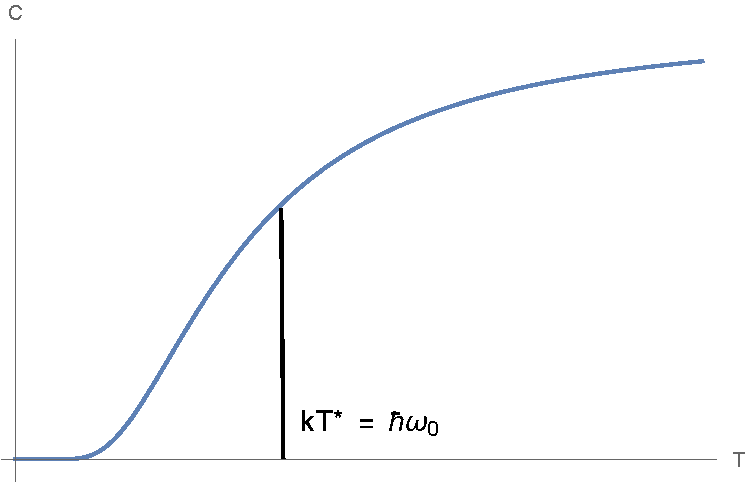
\includegraphics[width = 0.6\textwidth]{graphs/quantum_cc}
\end{figure}

\subsection{Photon gas and black-body radiation.}
\section{Bosons and fermions without interactions.}
\subsection{Indescernability and symetrisation.}
\subsection{Grand canonical partition function}
\section{Fermion gas.}
\section{Bosonic gas and condensation of Bose-Einstein.}

\end{document}